%\VignetteIndexEntry{PKgraph Overview}
%\VignetteDepends{PKgraph}
%\VignetteKeywords{PKgraph}
%\VignetteKeywords{PKgraph}
%\VignetteKeywords{PKgraph}
%\VignettePackage{PKgraph}
\documentclass[a4paper]{article}

\newcommand{\Rfunction}[1]{{\texttt{#1}}}
\newcommand{\Robject}[1]{{\texttt{#1}}}
\newcommand{\Rpackage}[1]{{\textit{#1}}}
\newcommand{\Rclass}[1]{{\textit{#1}}}
\newcommand{\Rmethod}[1]{{\textit{#1}}}

\author{Xiaoyong Sun$^\dagger$$^\ddagger$\footnote{johnsunx1@gmail.com}}

\usepackage{Sweave}
\begin{document}

\setkeys{Gin}{width=1\textwidth}

\title{User Guide for PKgraph Package}
\maketitle
\begin{center}$^\dagger$Binformatics and Computational Biology Program, $^\ddagger$Department of Statistics \\ Iowa State University, Ames, Iowa 50010, USA
\end{center}

\tableofcontents
%%%%%%%%%%%%%%%%%%%%%%%%%%%%%%%%%%%%%%%%%%%%%%

\section{Introduction}
Population pharmacokinetic (PopPK) modeling has become increasing important in
drug development because it allows unbalanced design, sparse data and the study
of individual variation. However, this complexity of the model makes it a challenge
to diagnose the fit.  Graphics can play an important and unique role in PopPK model diagnostics.
The software described in this paper, PKgraph, provides a graphical user interface for
PopPK model diagnosis with interactive graphics. It also provides an integrated and comprehensive platform for analysis
of pharmacokinetic data including exploratory data analysis, goodness of model fit,
model validation and model comparison. It can be used with a variety of modeling fitting software,
including NONMEM, Monolix, SAS and R. PKgraph is programmed in R, and uses the R packages
lattice, ggplot2 for static graphics, and rggobi for interactive graphics. This R package is
supported with a user-friendly graphical user interface so that users can easily control diagnosing
with simple clicks. The PKgraph software serves as a supplement to the existing packages:
NONMEM, Xpose and PsN for diagnosing models.
\newline
\newline
PKgraph is an R packaged built on the following R packages: RGtk2, gWidgets, gWidgetsRGtk2,
lattice, and ggplot2. It requires R ($>$ 2.0) and  GTK+, and runs under Windows, Linux and Mac.
\section{Installation}
PKgraph needs to install the following programs and R packages:
\newline \newline
1. install GTK \newline
For Windows, you can download the GTK Developer's Pack from
\newline
   http://gladewin32.sourceforge.net/
\newline
\newline
For Unix, you can fetch the source files for the different
libraries from
\newline
   ftp://ftp.gtk.org/pub/gtk/v2.8/
\newline
\newline
2. Install RGtk2 (Please see RGtk2 Installation notes if you have problems) \newline
\textit{install.packages(``RGtk2'')} \newline \newline
3. install rggobi   \newline
a. Download and install ggobi (www.ggobi.org)  \newline
b. Install rggobi: \textit{install.packages(``rggobi'')} \newline \newline
4. Install gWidgets  \newline
\textit{install.packages(``gWidgets'')} \newline \newline
5. Install cairoDevice \newline
\textit{install.packages(``cairoDevice'')} \newline \newline
6. Install gWidgetsRGtk2 \newline
\textit{install.packages(``gWidgetsRGtk2'')} \newline \newline
7. Install lattice  \newline
\textit{install.packages(``lattice'')} \newline \newline
8. Install ggplot2  \newline
\textit{install.packages(``ggplot2'')} \newline \newline
\section{PKgraph infrastructure}
The software incorporates a key concept: interactive graphics to link various datasets and diagnostics plots. The framework is programmed using RGtk2 and consists of main formats of interfaces,
(1) main, containing links to all parts of the software, and handles the basic data management, and links to diagnostic modules, and (2) graph, which provides tools specifically for each diagnostic module. 
\newline
\newline
\subsection{Graphical user interfaces}
\subsubsection{Main interface}
The main interface (Figure~\ref{c4_s2_1}) of PKgraph provide the links to all components of the software. There are four areas: (1) tool area (tool bar and menu bar, top), (2) directory area (middle-left), (3) data area (middle-right) and (4) status bar (bottom).
\newline
\newline
\begin{itemize}
	\item The tool area has menu items linking to the basic management modules (project, configuration, data management) and the diagnostic modules (exploratory data analysis, PK models, model validation, model comparison and interactive diagnostics). These are menu items containing numerous functions associated with each of the different types of diagnostics.
	\item The directory area shows current directory and all of its files. These files might be data files, or code, depending on the modeling software used.
	\item Clicking on any of the data files, will open them and display them in the data area (3).  Choosing the file also brings up a panel allowing for different formats to be read, thus handling all possible modeling software formats. The data files might contain raw data, and model diagnostics such as parameter estimates, fitted values and residuals and these are displayed in the table view of the data area.
	\item The stats bar displays the progress of the different functions, for example here it says ``Data is loaded successfully'' to indicate that there were no problems with opening the data file.
\end{itemize}
\begin{figure}[h!tb]
\centering
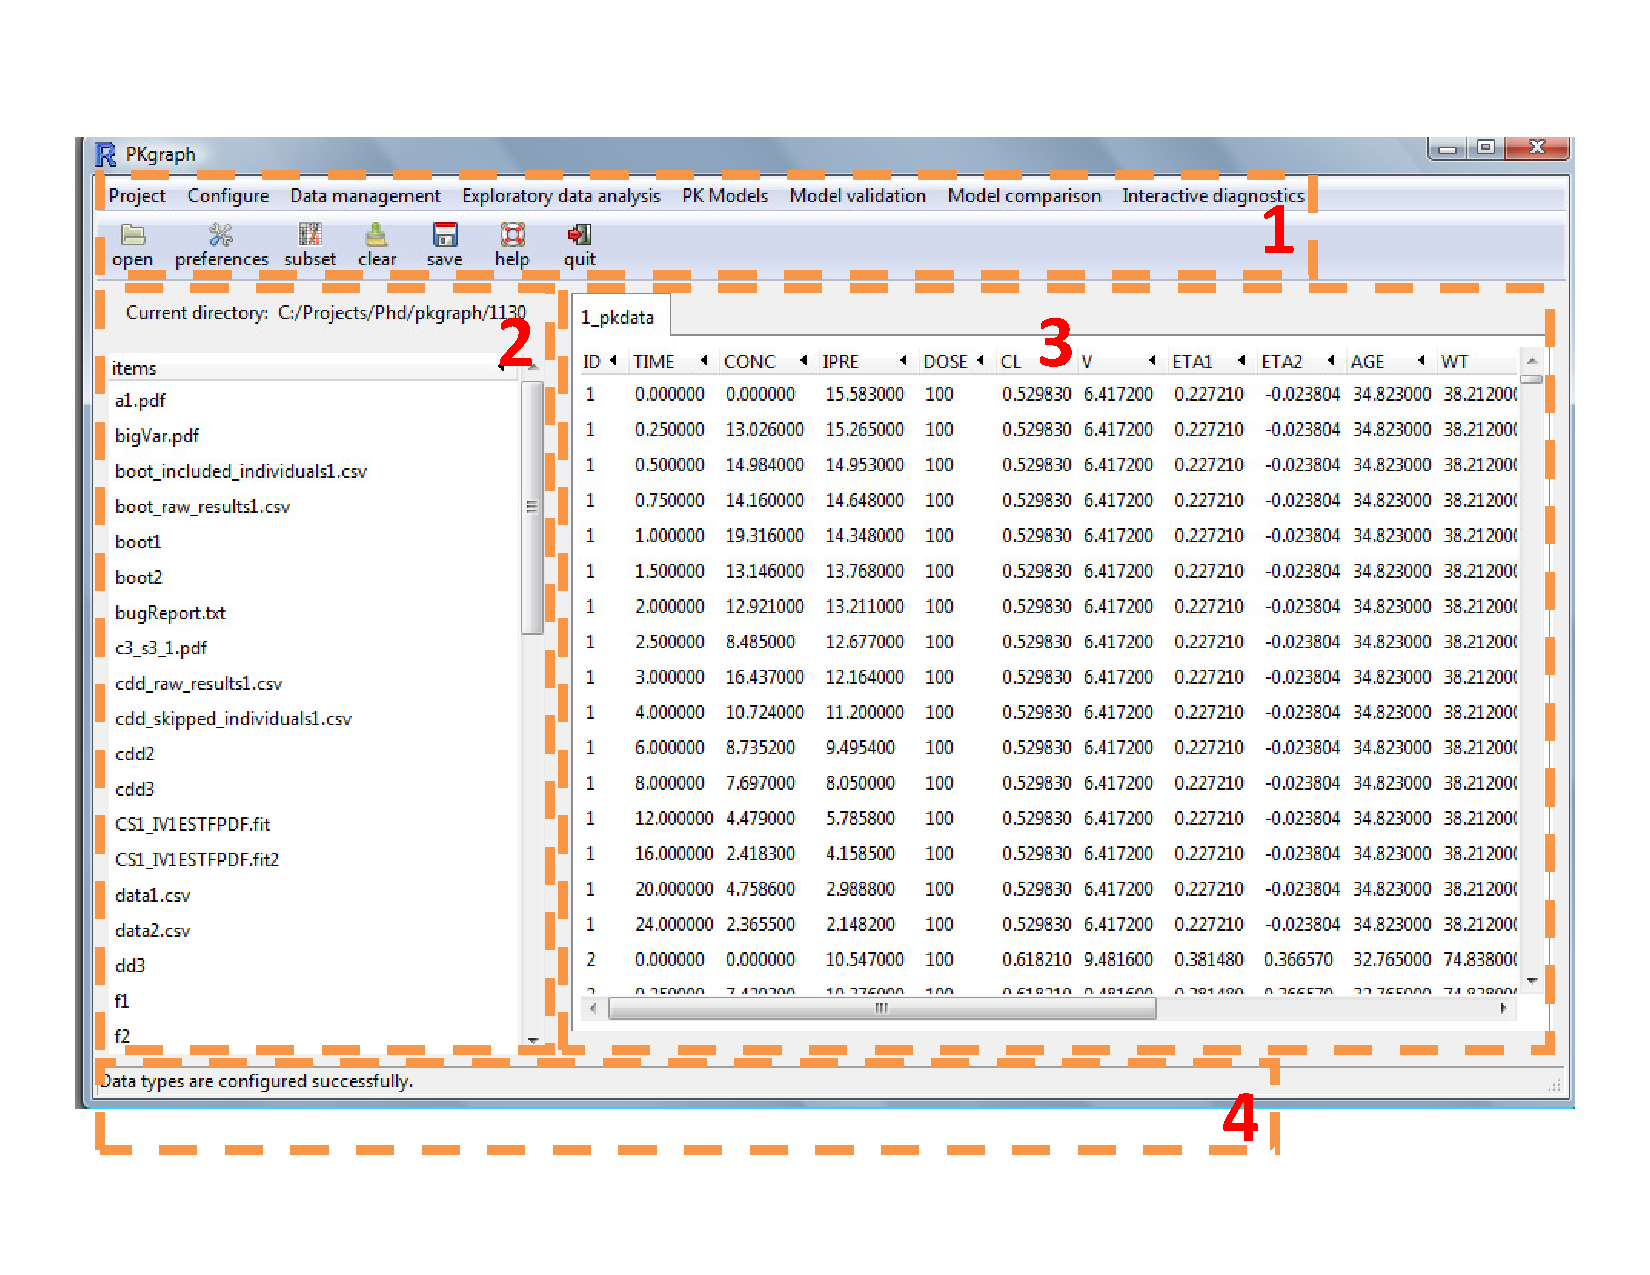
\includegraphics[scale=0.6]{c4_s2_1main.pdf}
\caption{Main interface of PKgraph}
\label{c4_s2_1}
\end{figure}
\subsubsection{Graph interface}
Selecting an item from a diagnostic module menu brings up a graph interface (Figure~\ref{c4_s2_2}). The style of the interface is the same for all diagnostic functionality.  It contains three areas: 1) parameter setup area, 2) tool bar, 3) plot area.
\newline
\newline
\begin{itemize}
	\item The parameter area setup allows choice of variable, plot labels, layout for trellis or facetted plots. A choice of lattice or ggplot2 graphics is provided.  Note: At the bottom of this area, there is a module called ``command area'', which is for next release. It is not fully functional at this point.
	\item The tool bar allows users to 1) save plots, 2) open plots for interactive graphics (\textbf{ctrl + b for brushing data}), 3) display subset selection from ggobi, 4) save subset selection from ggobi and 5) close ggobi.
		\begin{itemize}
			\item save plots: this button can save the current plot from \textbf{plot area}. The figure can be saved as pdf, jpg, tiff, png formats. This format is configured by \textit{Set saving format} in the \textit{Configure} menu item. For multiple plots generated with one parameter set, such as plots for observation concentration versus time conditioned on 50 patients, R will only keep the last few patients as one page in the \textbf{plot area}. This button will automatically save all pages for all patients with the specified figure format.
			\item open plots for interactive graphics: this button opens two plots in ggobi for interactive graphics. The first plot is a time series plot for this data (observed concentration versus time), and the second plot is the current plot from \textbf{plot area}. These two plots are linked by patient ID. A specific feature of interactive graphics is to explore data by brushing. In the ggobi, users can use \textbf{ctrl + b for brushing data} to link two plots. For those who would like to use more advanced features of interactive graphics, ggobi manual is a good resource (http://www.ggobi.org/).
			\item display subset selection from ggobi: this button helps user to visualize and analyze the brushed data from the previous step: \textit{ open plots for interactive graphics}. The brushed data is shown as a new dialog.
			\item save subset selection from ggobi: this buttons save all brushed data from previous step: \textit{open plots for interactive graphics}, \textit{ display subset selection from ggobi}. 
			\item close ggobi: close all related ggobi instances.
		\end{itemize}
	\item The plot area displays the figure, and multiple figures if more than one are created.
\end{itemize}
\begin{figure}[h!tb] \centering
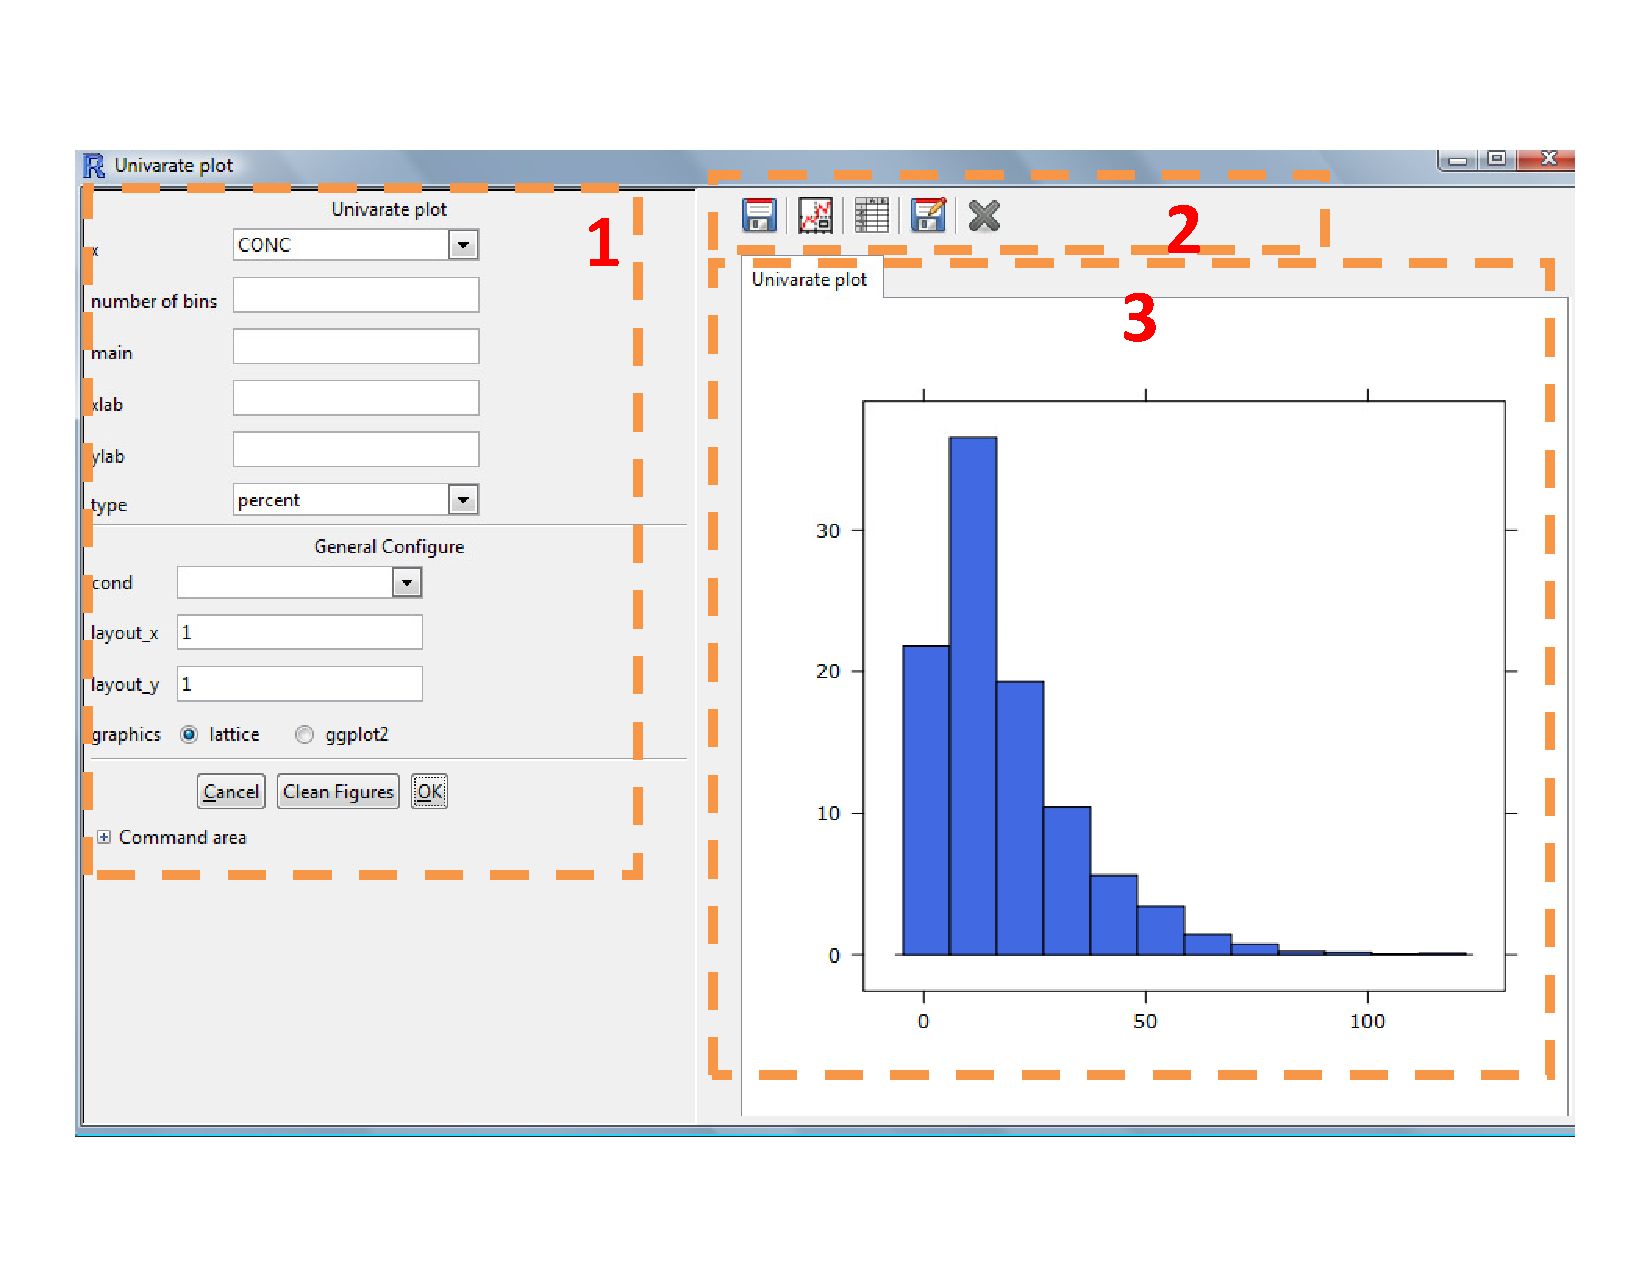
\includegraphics[scale=0.6]{c4_s2_2graph.pdf}
\caption{Graph interface of PKgraph}
\label{c4_s2_2}
\end{figure}
\subsection{Functional module}
Functional module matches the menu items in PKgraph toolbar. It includes the following menu itmes: \newline
\begin{itemize}
	\item Project
	\item Configure
	\item Data management
	\item Exploratory data analysis
	\item PK models
	\item Model validation
	\item Model comparison
	\item Interactive graphics
\end{itemize}
In the next sections, I will go through each menu item in detail.
\section{Quick start}
PKgraph targets audiences working in population pharmacokinetics models,
and particularly those professionals who have only basic knowledge of R.
\subsection{Input data}
\subsubsection{data.frame}
PKgraph accepts one type of input data: data.frame. It can be model fit results from NONMEM, Monolix, SAS or R. This data.frame should include ID, time, observed concentration, individual predicated concentration, population predicted concentration, residuals, weighted residuals, parameters, random effects, etc. Details are as follows. Note: Abbreviated terms are explained in Table~\ref{tnew_function_1}.
\begin{itemize}
	\item Exploratory data analysis: ID, Time, CONC 
	\item PK models: See details in Table~\ref{c2_s3_t12}. 
	\item Model comparison: ID, Time, CONC, and interested variables from fit results, such as WRES, IPRE, etc. For this module, two data.frames come from two model fit results are required.
\end{itemize}
Dependent on the modeling software, users need to convert the model fit results to this single data.frame. After that, PKgraph can read in and diagnose the model fit results. For NONMEM, the \textit{tab} file can be considered as this single data.frame, and read in R directly. For Monolix, there are a few output files, and users have to combine them as one single file, including all the interested variables.
\newline
\newline
An sample data from NONMEM,
\begin{verbatim}
> library(PKgraph)
> data(pkdata)
\end{verbatim}
\subsubsection{NONMEM folders}
For model validation, PKgraph accepts two kinds of model validation data: 1) results from PsN; 2) results from multiple NONMEM runs. For the first type of data, PsN has the following functions: bootstrap, case deletion and stochastic simulation. PKgraph provides the graphic ability to visualize the final results from PsN. For the second type of data, PKgraph can handle multiple NONMEM run folders and extract useful information to visualize.
Please see details in \textbf{Model validation}.
\subsection{Diagnose model}
There are eight function menu items in the \textbf{main interface}. 
Each matches a functional module. They can be considered as two categories: 
\textbf{basic} and \textbf{diagnostic} modules. 
The basic module includes ``Project'', ``Configure'', ``Data management'' menu items, 
and the diagnostic module includes ``Exploratory data analysis'', ``PK model'', 
``Model validation'', ``Model comparison'', ``Interactive graphics'' menu items. 
The five menu items in the diagnostic module can be utilized separately.  
\newline
\newline
The basic module is utilized to read in data, configure data and manage data. The diagnostic module aims to test assumptions of population pharmacokinetic models. Please see the following section for details.
\newline
\newline
The workflow of diagnosing models is as follows, 

\subsection{Basic graphical parameters}
In PKgraph, we use a lot of popular arguments from R graphics. Here is the explanation. For those who want to know more about these parameters, please check R manual.
\begin{table}[h!tb] \centering
\begin{tabular}{l l} \hline
\textbf{ Abbreviated terms} & \textbf{Description}  \\ \hline
main & main title of the plot. It is the argument in R functions.\\
xlab/ylab & label of the x/y axis. It is the argument in R functions. \\
type & what type of plot should be drawn \\
layout\_x & the number of columns in a multi panel display \\
layout\_y & the number of rows in a multi panel display \\
cond & conditional variable \\
loess/lowess & locally weighted scatterplot smoothing \\
\hline
\end{tabular}
\caption{Basic graphical parameters}
\label{tnew_function_2}
\end{table}

\subsection{Abbreviations in the software}
\begin{table}[h!tb] \centering
\begin{tabular}{l l} \hline
\textbf{ Abbreviated terms} & \textbf{Description}  \\ \hline
ID & Patient ID \\
TIME & Time after dose \\
CONC & Observed concentration of drug in the body \\
PRED & Population predicted concentration \\
RES & Residual \\
WRES & Weighted residual \\
IPRED & individual predicted concentration \\
IWRES & Individual weighted residual \\
COV & Covariates \\ 
DV & Dependent variables (Usually observed concentration) \\
IDV & Independent variables (Usually time) \\
\hline
\end{tabular}
\caption{Abbreviated terms}
\label{tnew_function_1}
\end{table}
The abbreviated variables used in the software are listed as Table~\ref{tnew_function_1}.

\section{Menu items in main interface}
In this section, I will go through each function in the menu items of toolbar.
\subsection{Project}
This menu item is in charge of input, output and save data. It has the following functions (Figure~\ref{project}),
\begin{itemize}
	\item \textit{Open data}: open modeling fit result from NONMEM, Monolix, SAS, R or other software.
  It has options to setup the data format, start line and separation symbol.
	\item \textit{Save a file}: save a file.
	\item \textit{Save a workspace}: save a workspace for later usage. It generally saves a group of lists
	for configuration and related data.
	\item \textit{Clean data}: clean all loaded data.		
	\item \textit{Restore old workspace}: restore the workspace from the data and list you saved from previous step.
	\item \textit{Exit}: exit from PKgraph.
\end{itemize}
\begin{figure}[h!tb] \centering
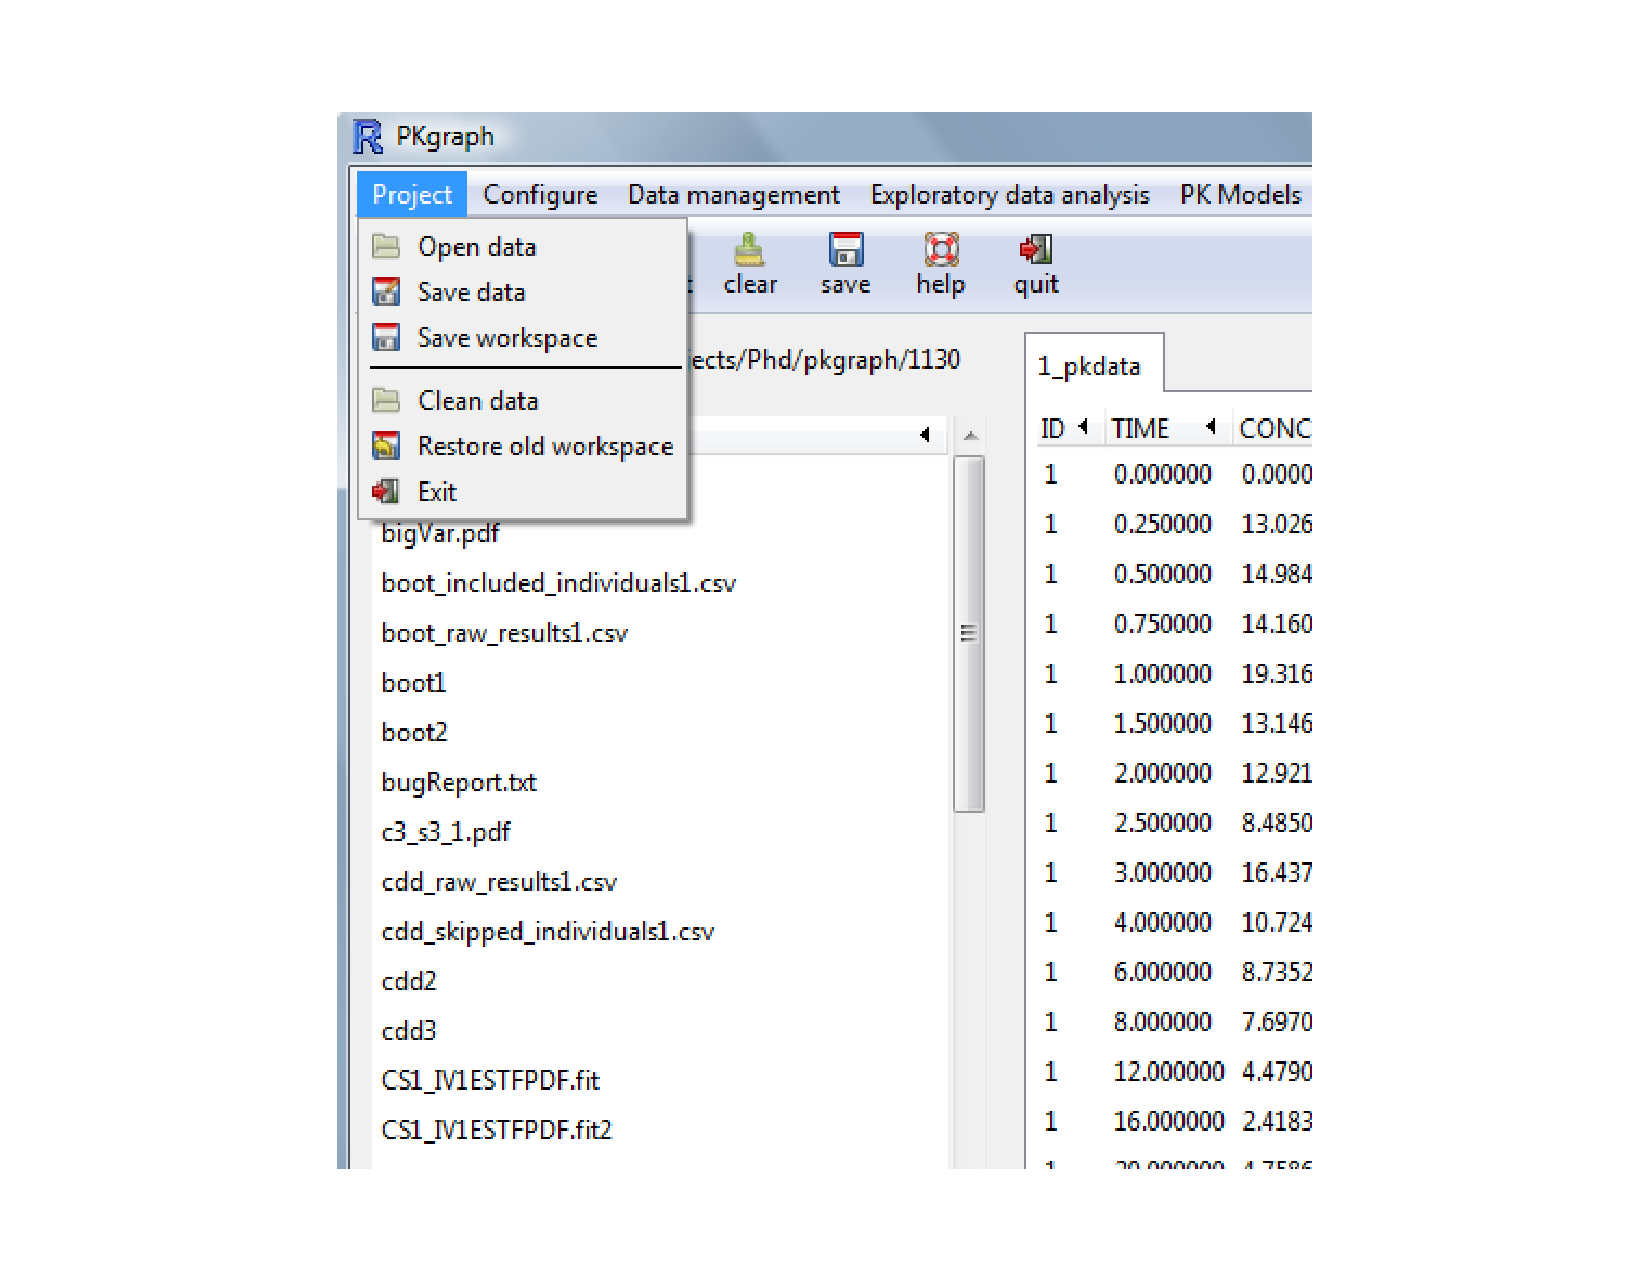
\includegraphics[scale=0.6]{project.pdf}
\caption{Menu items in \textit{Project}}
\label{project}
\end{figure}
\subsection{Configure}
This menu itme is utilized to configure PKgraph. It has the following functions (Figure~\ref{configure}),
\begin{itemize}
	\item \textit{Set data type}: set the ID, TIME, CONC variables for current PK data. This configuration is used for integrative graphics to draw a time series plot automatically.
	\item \textit{Set working directory}: change current working directory in R.
	\item \textit{Set saving format}: set up saving format for figures, including pdf, jpg, tiff, png
  bmp, win.metafile, and figure width and height. If figure width and height is not 
  configured, the default one will be used. 
  Note: to save figure in \textbf{graph interface}, users need to configure this menu 
  first. 
  \item \textit{Set figure configuration}: color and loess can be selected for figures.
\end{itemize}
\begin{figure}[h!tb] \centering
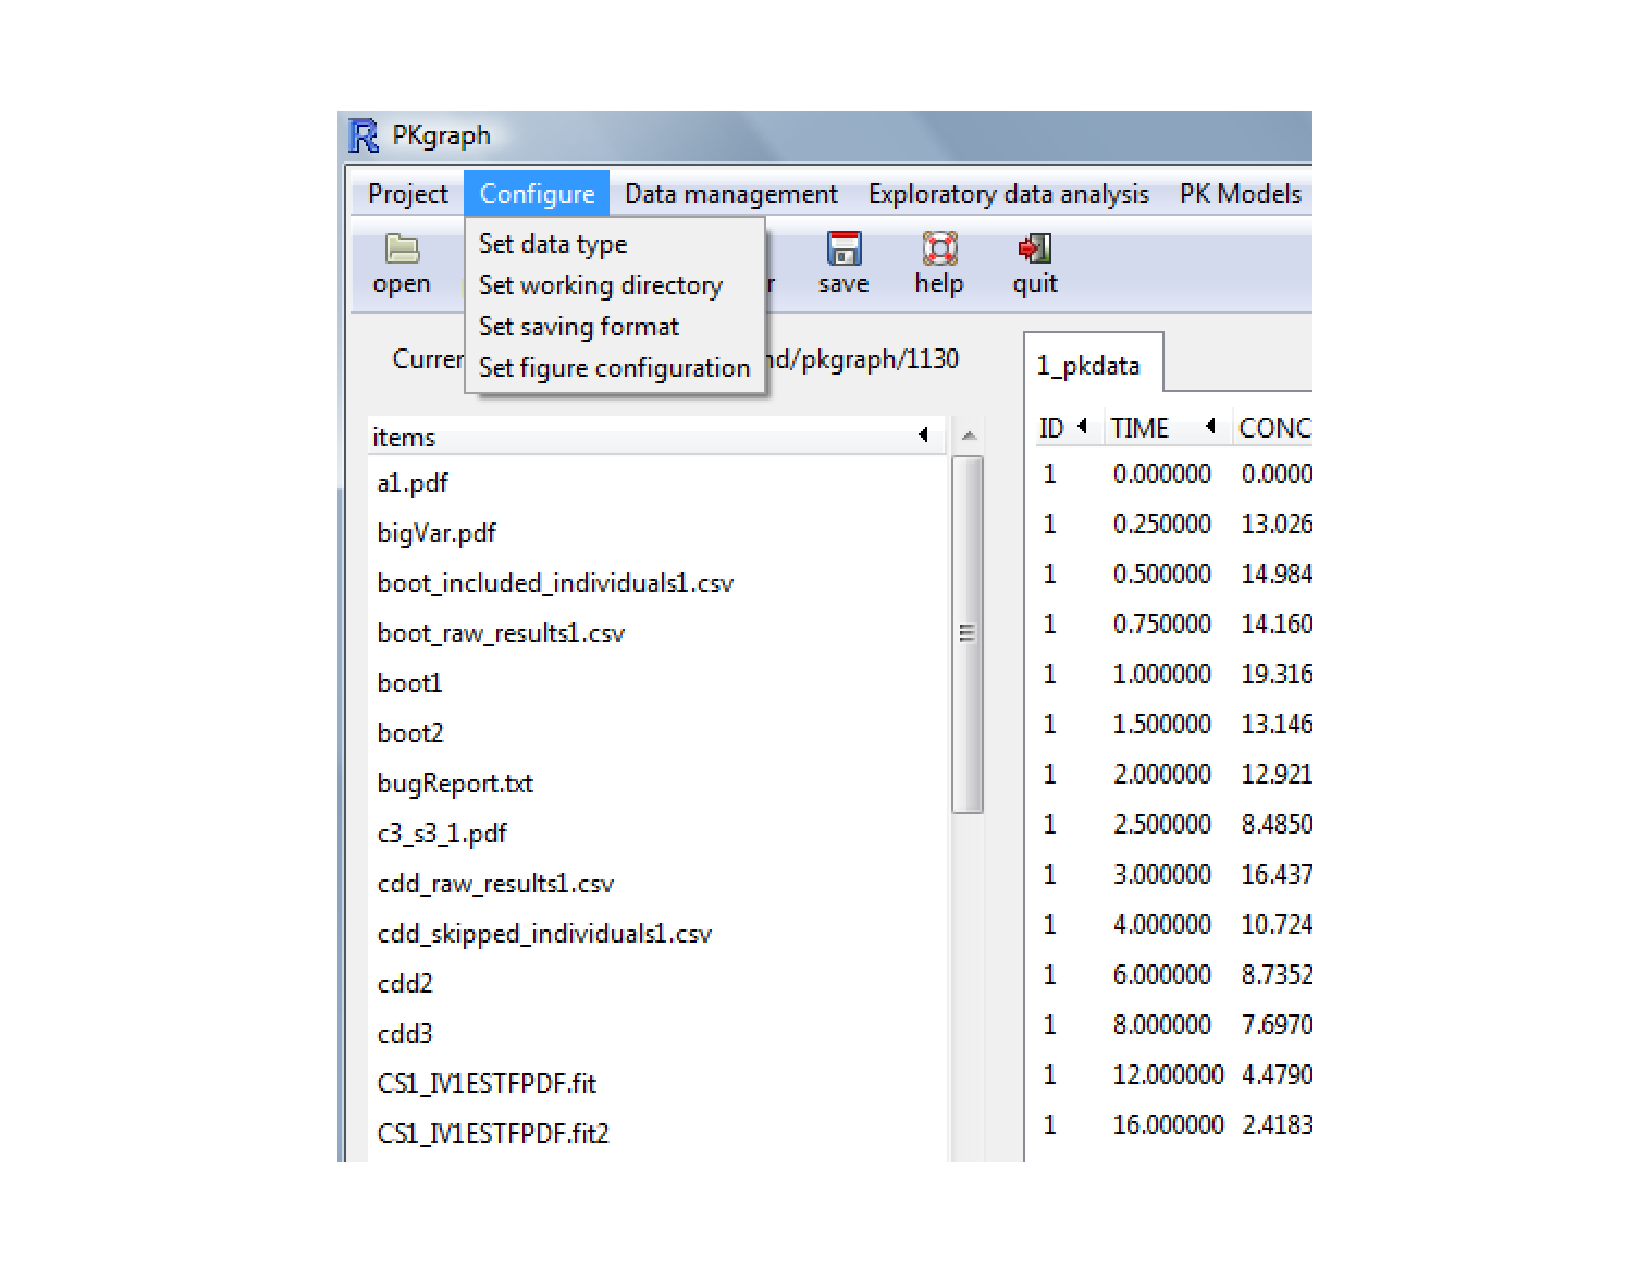
\includegraphics[scale=0.6]{configure.pdf}
\caption{Menu items in \textit{Configure}}
\label{configure}
\end{figure}
\subsection{Data management}
This menu item is utilized to manage data. It has the following functions (Figure~\ref{data}),
\begin{itemize}
	\item \textit{Subset}: subset current data. After this, a new subset data will generate in the \textbf{data area} of \textbf{main interface}. And it will be the current working data for the following diagnosis. If users do not want to work on this data, users can click the tab of \textbf{data area} and select the proper one as the current working data.
	\item \textit{Factor}: factor categorical variables. 
	Graphical packages require the variable to be factor type in order to 
	display the categorical symbol in figures.	
	For example, in Figure~\ref{modelcc2}, after we make the ``ISM'' as a factor, 
	the symbol ``0/1'' is show as the subtitle on the figure; otherwise, 
	the name of variable ``ISM''
	will be shown instead.
\end{itemize}
\begin{figure}[h!tb] \centering
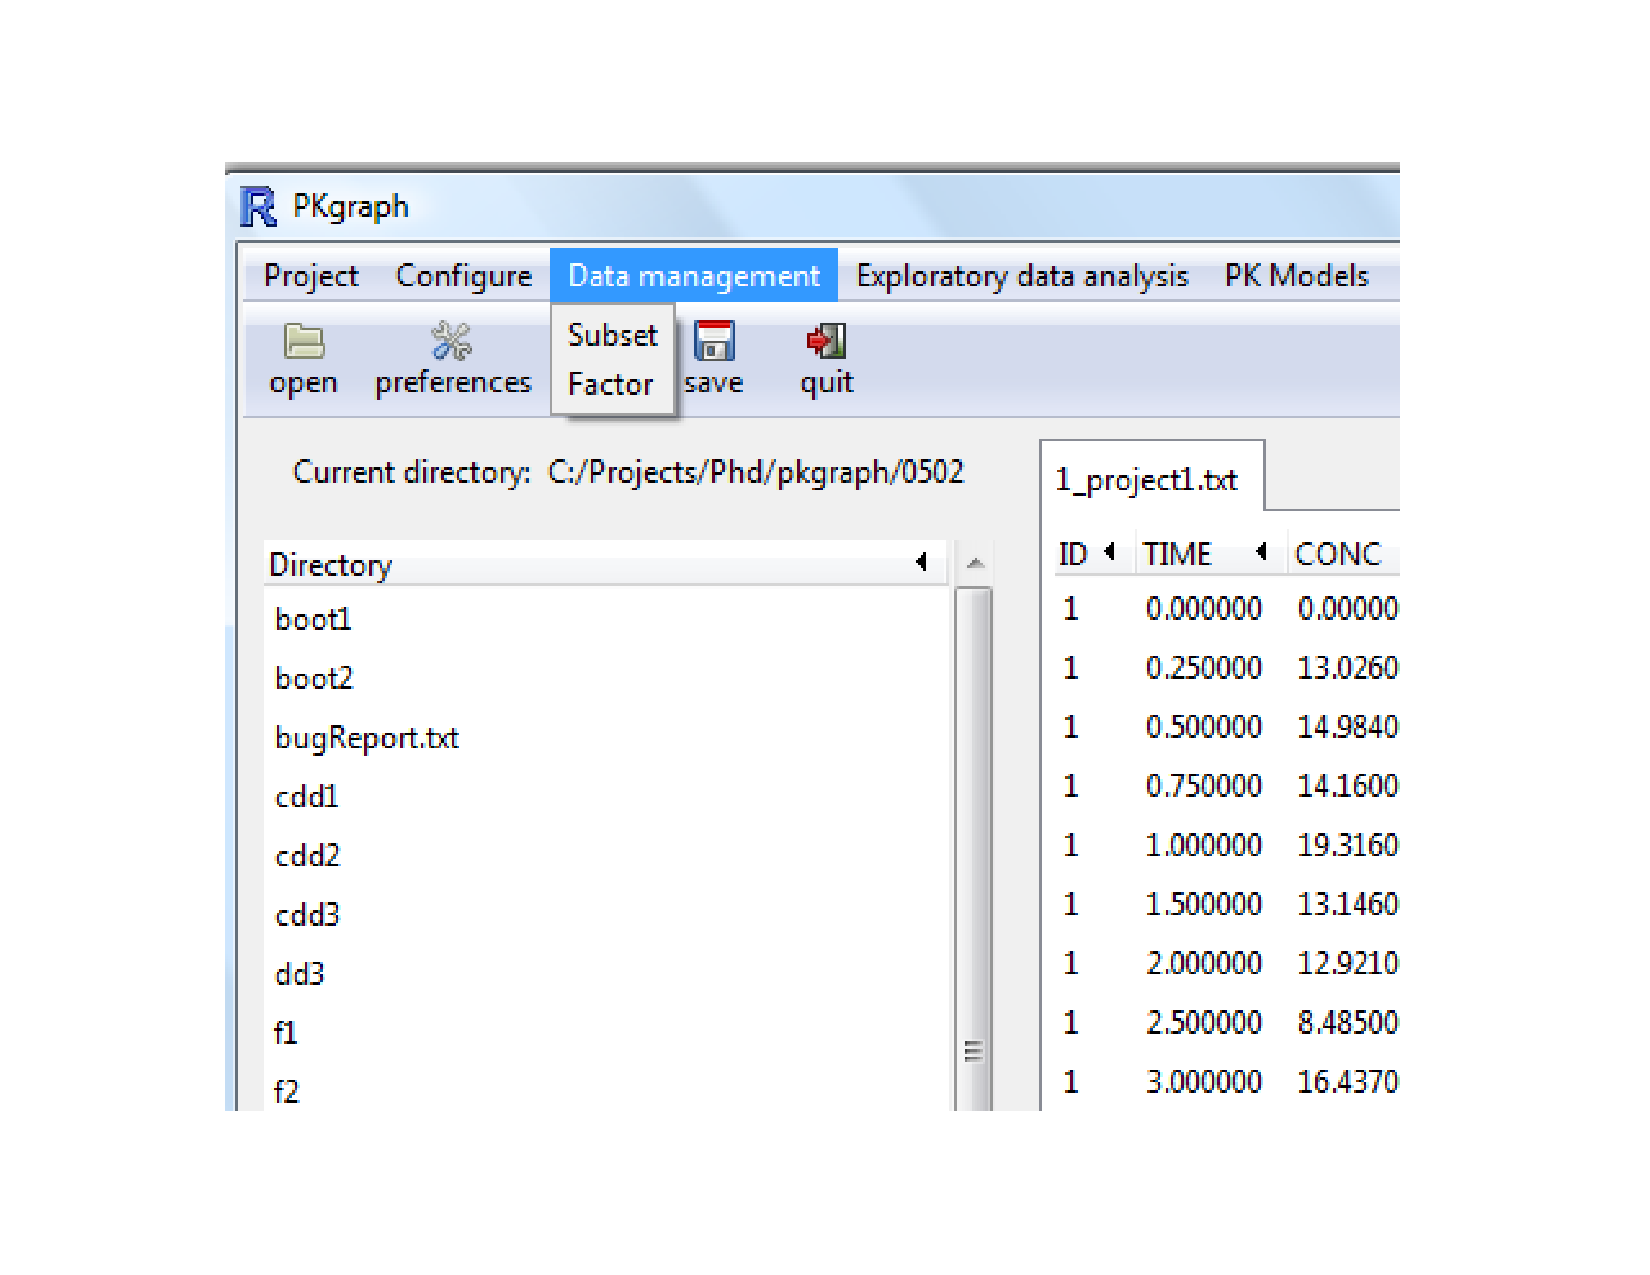
\includegraphics[scale=0.6]{data.pdf}
\caption{Menu items in \textit{Data management}}
\label{data}
\end{figure}
\subsection{Exploratory data analysis}
This menu item is utilized to explore data and screen patterns. 
The explanation for the basic parameter set is available at section: \textbf{Basic graphical parameters}.
It has the following functions (Figure~\ref{eda}),
\begin{itemize}
	\item \textit{Univariates}: plot univariate varaiables. 
	\item \textit{Bivariates}: plot bivariate variables.
	\item \textit{Parallel coordinate plot}: Parallel coordinate plot for multivariate variables.
	\item \textit{Scatterplot matrix}: Scatterplot matrix for multivariate variables.
\end{itemize}
\begin{figure}[h!tb] \centering
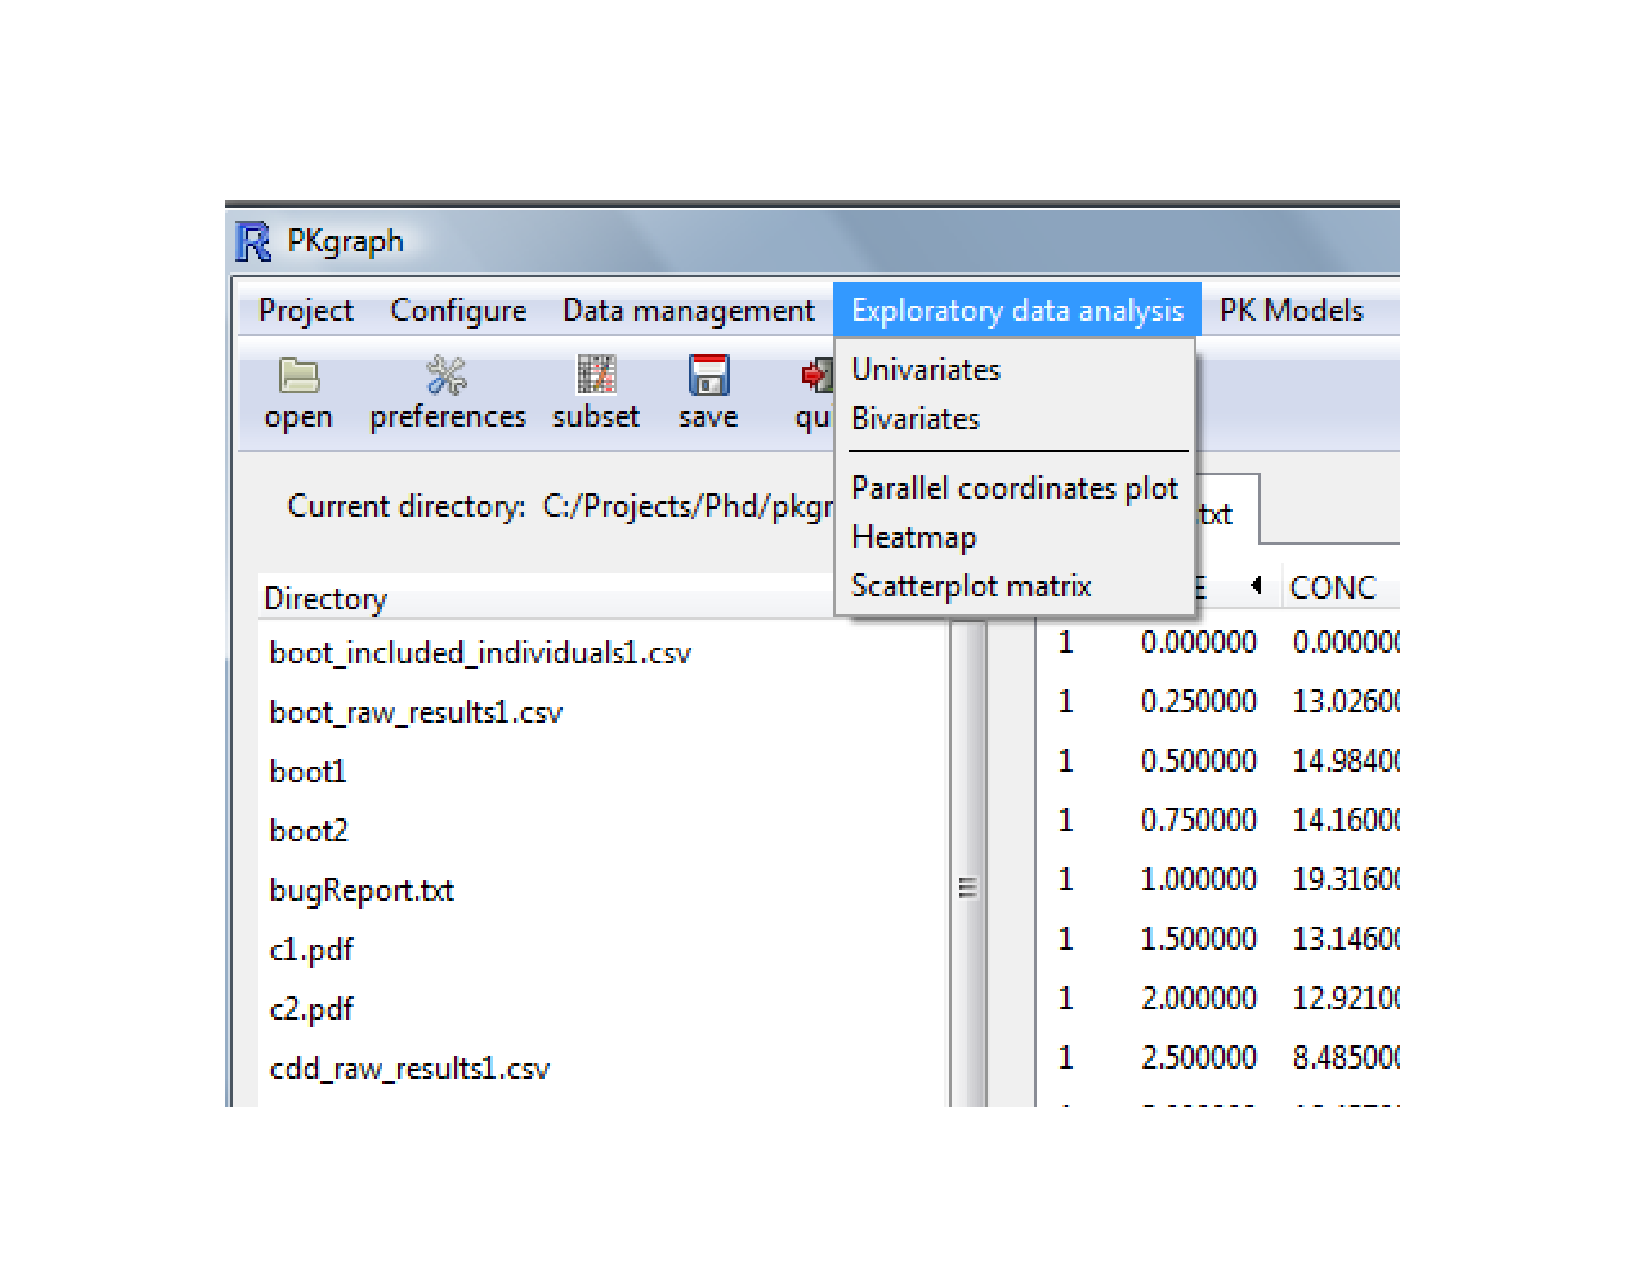
\includegraphics[scale=0.6]{eda.pdf}
\caption{Menu items in \textit{Exploratory data analysis}}
\label{eda}
\end{figure}
\subsubsection{Univariate}
When clicking this menu item, users will generate a 
\textbf{graph interface}(Figure~\ref{c4_s2_2}). In this interface, users can 
specify all parameters in the left area of window. In the right area of window, 
it has five buttons on the top explained in section: \textbf{Graph interface}.
\subsubsection{Bivariate}
This menu item also generates a ``graph interface''. It is similar to the Univariate interface, except that users will have two variables instead of one.
\subsubsection{Parallel coordinate plots}
This menu item provides access to \textit{parallel} function from lattice package.
\subsubsection{Scatterplot matrix}
This menu item provides access to \textit{splom} function from lattice package.
%%%%%%%%%%%%%%%%%%%%%%%%%%%%%%%%%%%%%%%%%%%%%%%%%%%%%%%%%%%
\subsection{PK models}
This menu item is utilized to check model assumptions and goodness of fit. The guideline follows Census menu (http://census.sourceforge.net/). It has the eight functions (Figure~\ref{pkmodel}). \textbf{ Configure model result} is required for the other seven functions. 
Users have to configure data variable first before going to specific model diagnostics.
\begin{figure}[h!tb] \centering
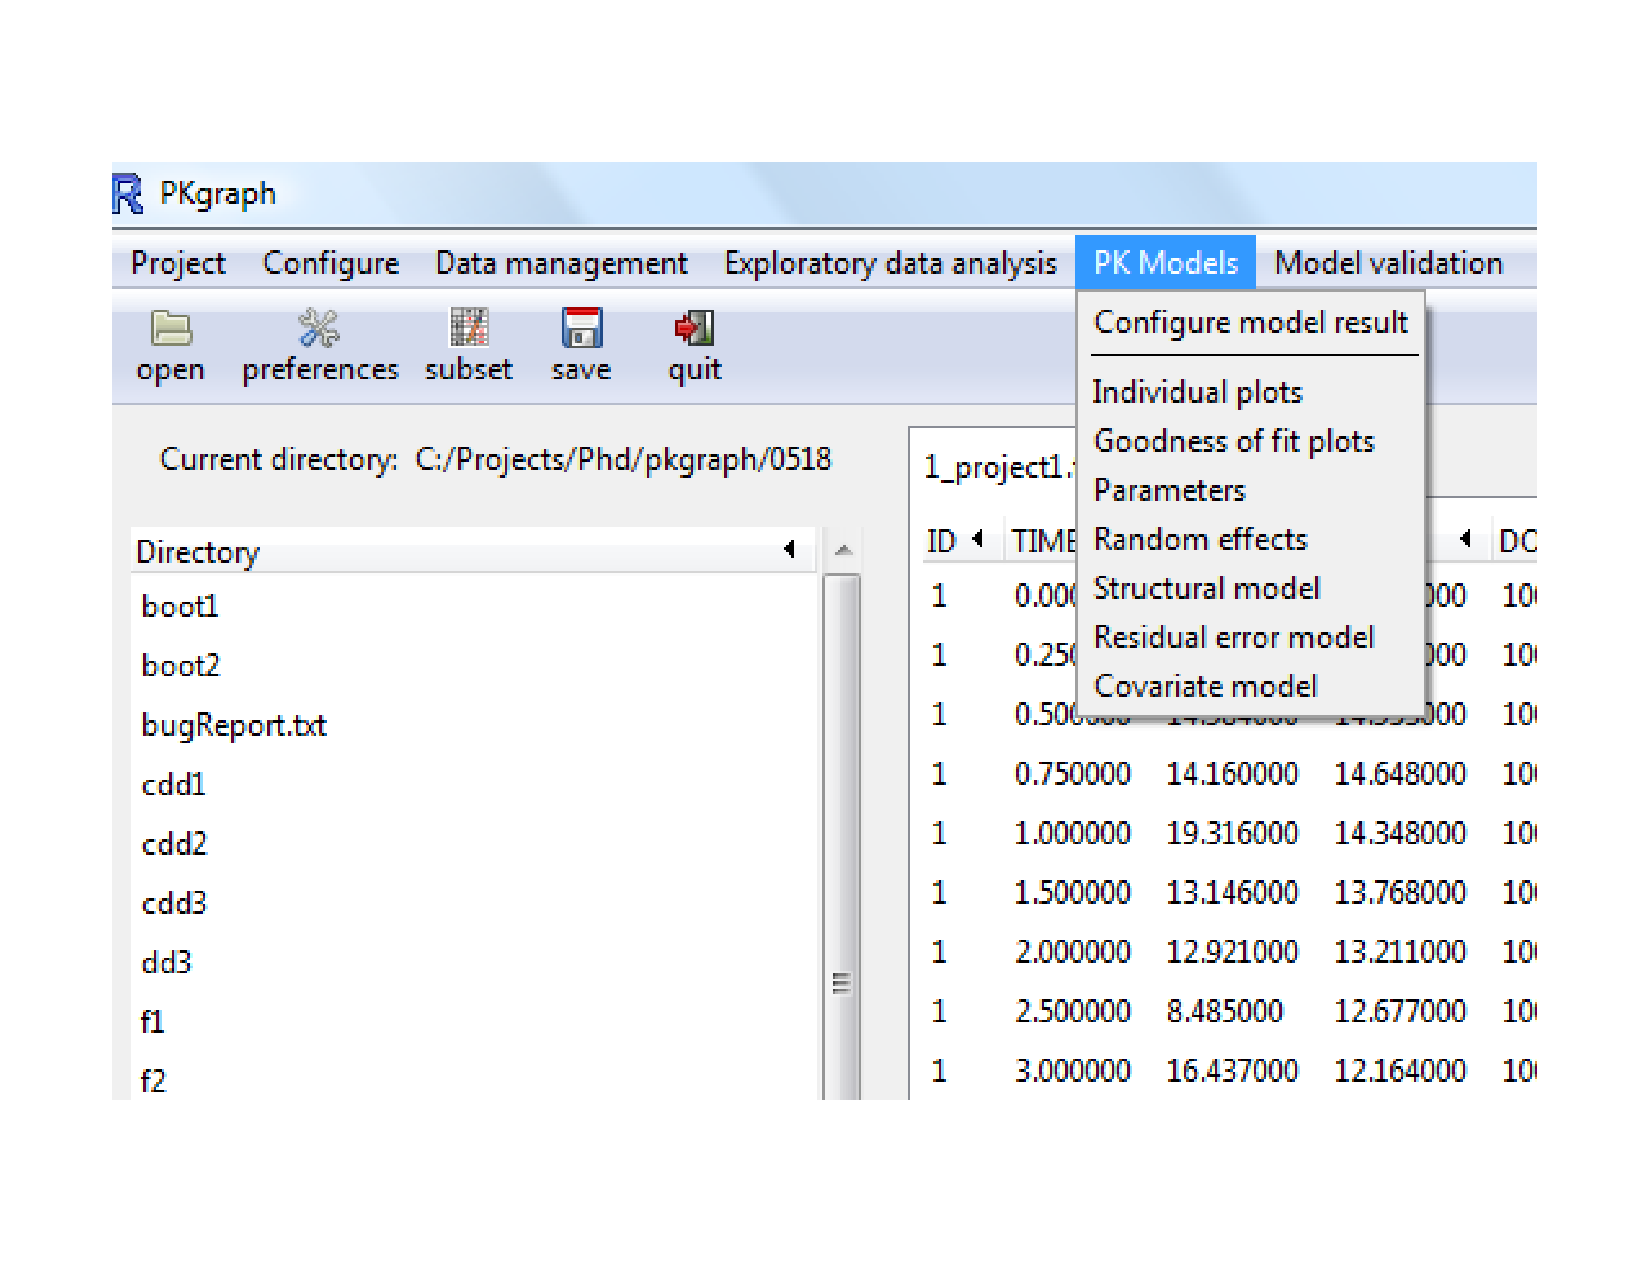
\includegraphics[scale=0.6]{pkmodel.pdf}
\caption{Menu items in \textit{PK models}}
\label{pkmodel}
\end{figure}
%%%%%%%%%%%%%%
\subsubsection{Configure model result}
This is the key step to match data variables to default metric system. By this step, fit results from any platform (NONMEM, Monolix, SAS, R) can be interpreted graphically in figures.
\begin{figure}[h!tb] \centering
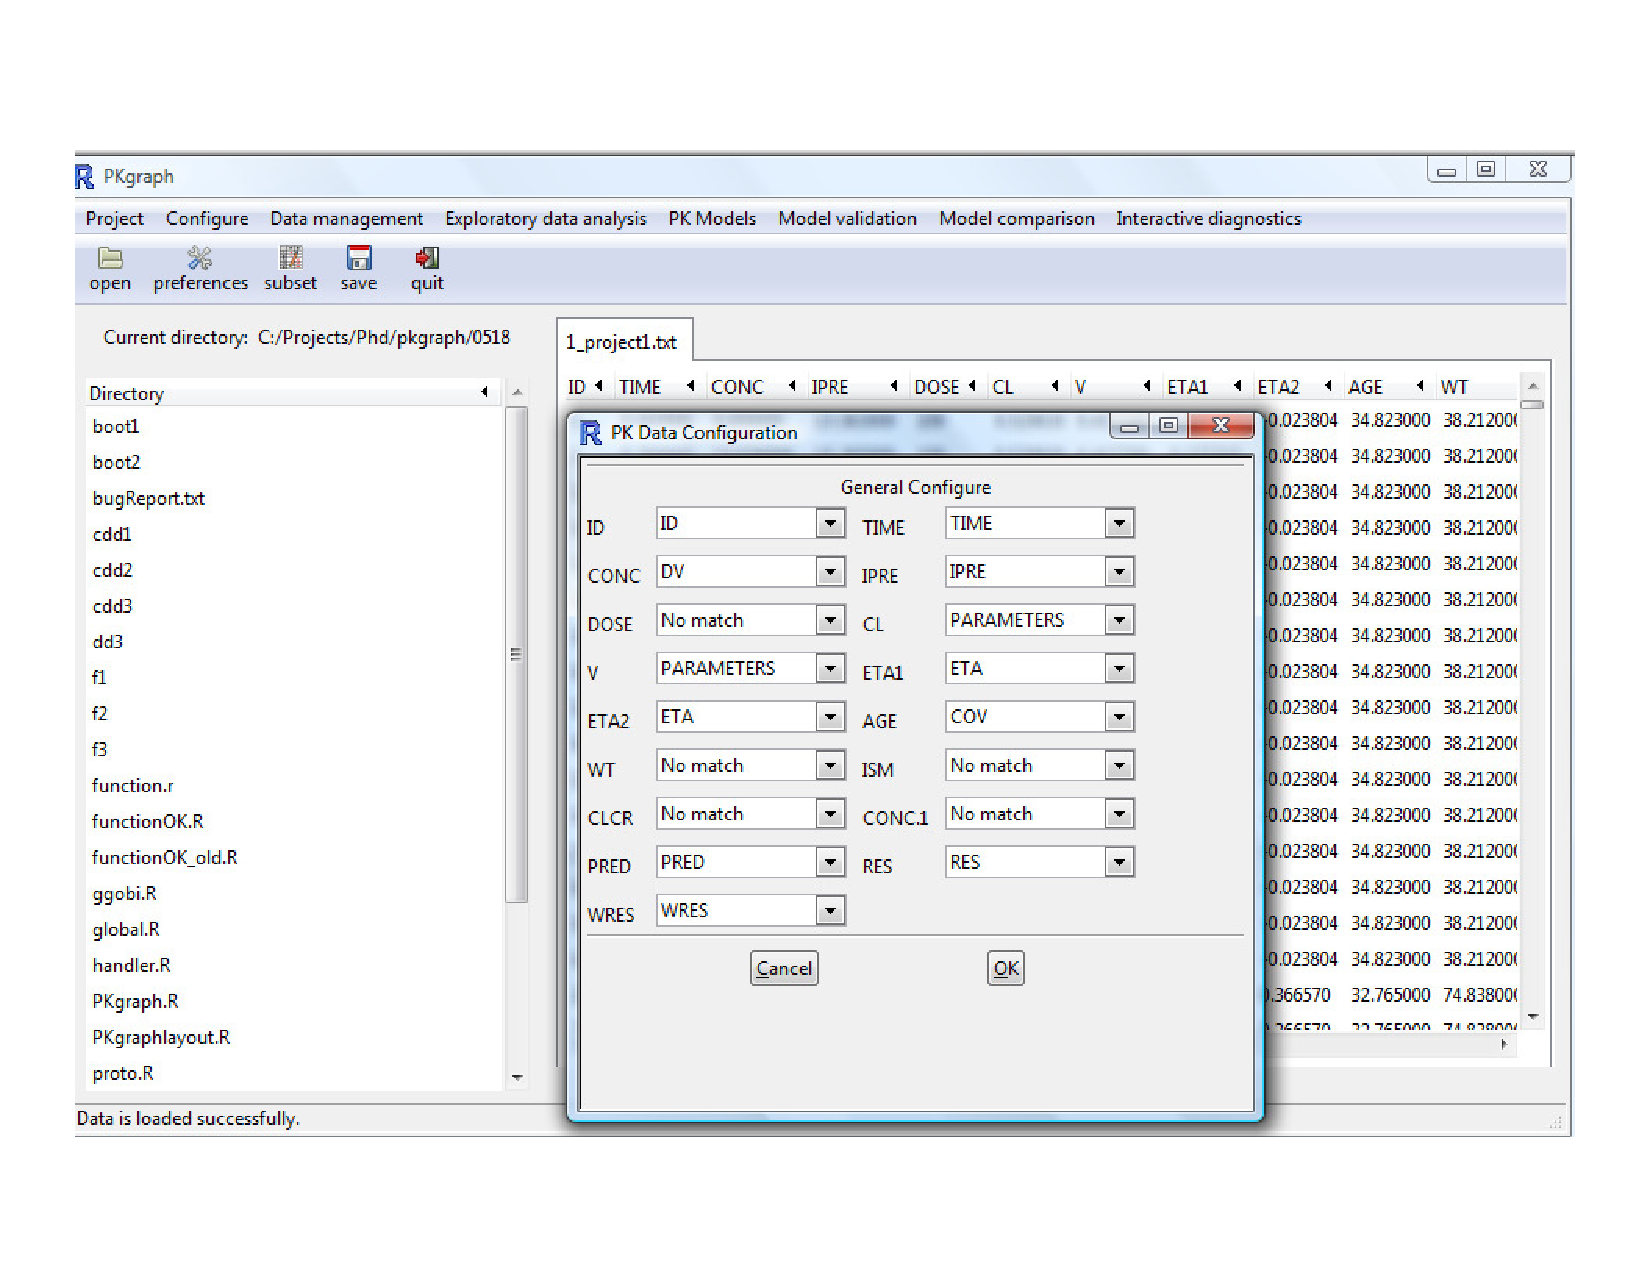
\includegraphics[scale=0.6]{pkmodel_config.pdf}
\caption{\textit{Configure model result} in \textit{PK models}}
\label{pkmodel_config}
\end{figure}
\begin{table}[h!tb] \centering
% Use: \begin{tabular{|lcc|} to put table in a box
\begin{tabular}{lcc} \hline
\textbf{Package variable} & \textbf{Description}  \\ \hline
ID & Patient ID \\
TIME & Time after dose \\
CONC & Observed concentration of drug in the body \\
PRED & Population predicted concentration \\
RES & Residual \\
WRES & Weighted residual \\
IPRED & individual predicted concentration \\
IWRES & Individual weighted residual \\
COV & Covariates \\ 
DV & Dependent variables \\
IDV & Independent variables \\
\hline
\end{tabular}
\caption{Package metric system}
\label{c2_s3_t1}
\end{table}
\newline
\newline
The interface for this function is shown in Figure~\ref{pkmodel_config}. The fixed column (left) is column name from data, and the selectable column (right) is variable name from the default metric system (Table~\ref{c2_s3_t1}). By this matching, the other seven functions can be performed. However, these functions work independently, and some variables in the default metric system must be matched to those in real data (Table~\ref{c2_s3_t12}).

\begin{table}[h!tb] \centering
\begin{tabular}{ll} \hline
\textbf{Functions} & \textbf{Required items to be selected in right column}  \\ \hline
\textbf{Individual plots} & ID \\
\textbf{Basic goodness of fit plots} & PRED, IPRE, DV, IDV, WRES \\
\textbf{Parameters} & PARAMETERS \\
\textbf{Structural model} & PRED, IPRE, DV, IDV, WRES, COV \\
\textbf{Residual error model} & WRES, PRED, COV, IPRE \\
\textbf{Covariate model} & PARAMETERS, ETA, WRES, COV \\
\textbf{Random effects} & ETA \\
\hline
\end{tabular}
\caption{Required variables for different functions}
\label{c2_s3_t12}
\end{table}
%%%%%%%%%%%%%%
\subsubsection{Individual plots}
Bivariate plot for each individual.
\subsubsection{Basic goodness of fit plots}
Goodness of fit plot is one of key tools to check model fitting. 
These kinds of plots will give an overall perspective of model performance, 
including scatter plot for concentration versus PRED, concentration versus IPRED, 
PRED versus IDV (time) and IPRED versus IDV (time).
%%%%%%%%%%%%%%
\subsubsection{Parameters}
Generally, there are assumptions for distribution of parameters during modeling process. The histogram is utilized to check this distribution. In addition, the correlation of parameters has significant effect on modeling performance, and it can be checked by scatter plots or a scatterplot matrix.
\newline
\newline
The interface for this function is shown in Figure~\ref{pkmodel_para}. After users choose proper parameters in the left window, the system will produce all figures automatically. Users can pick specific figures for diagnosing with functions in the toolbar.\begin{figure}[h!tb] \centering
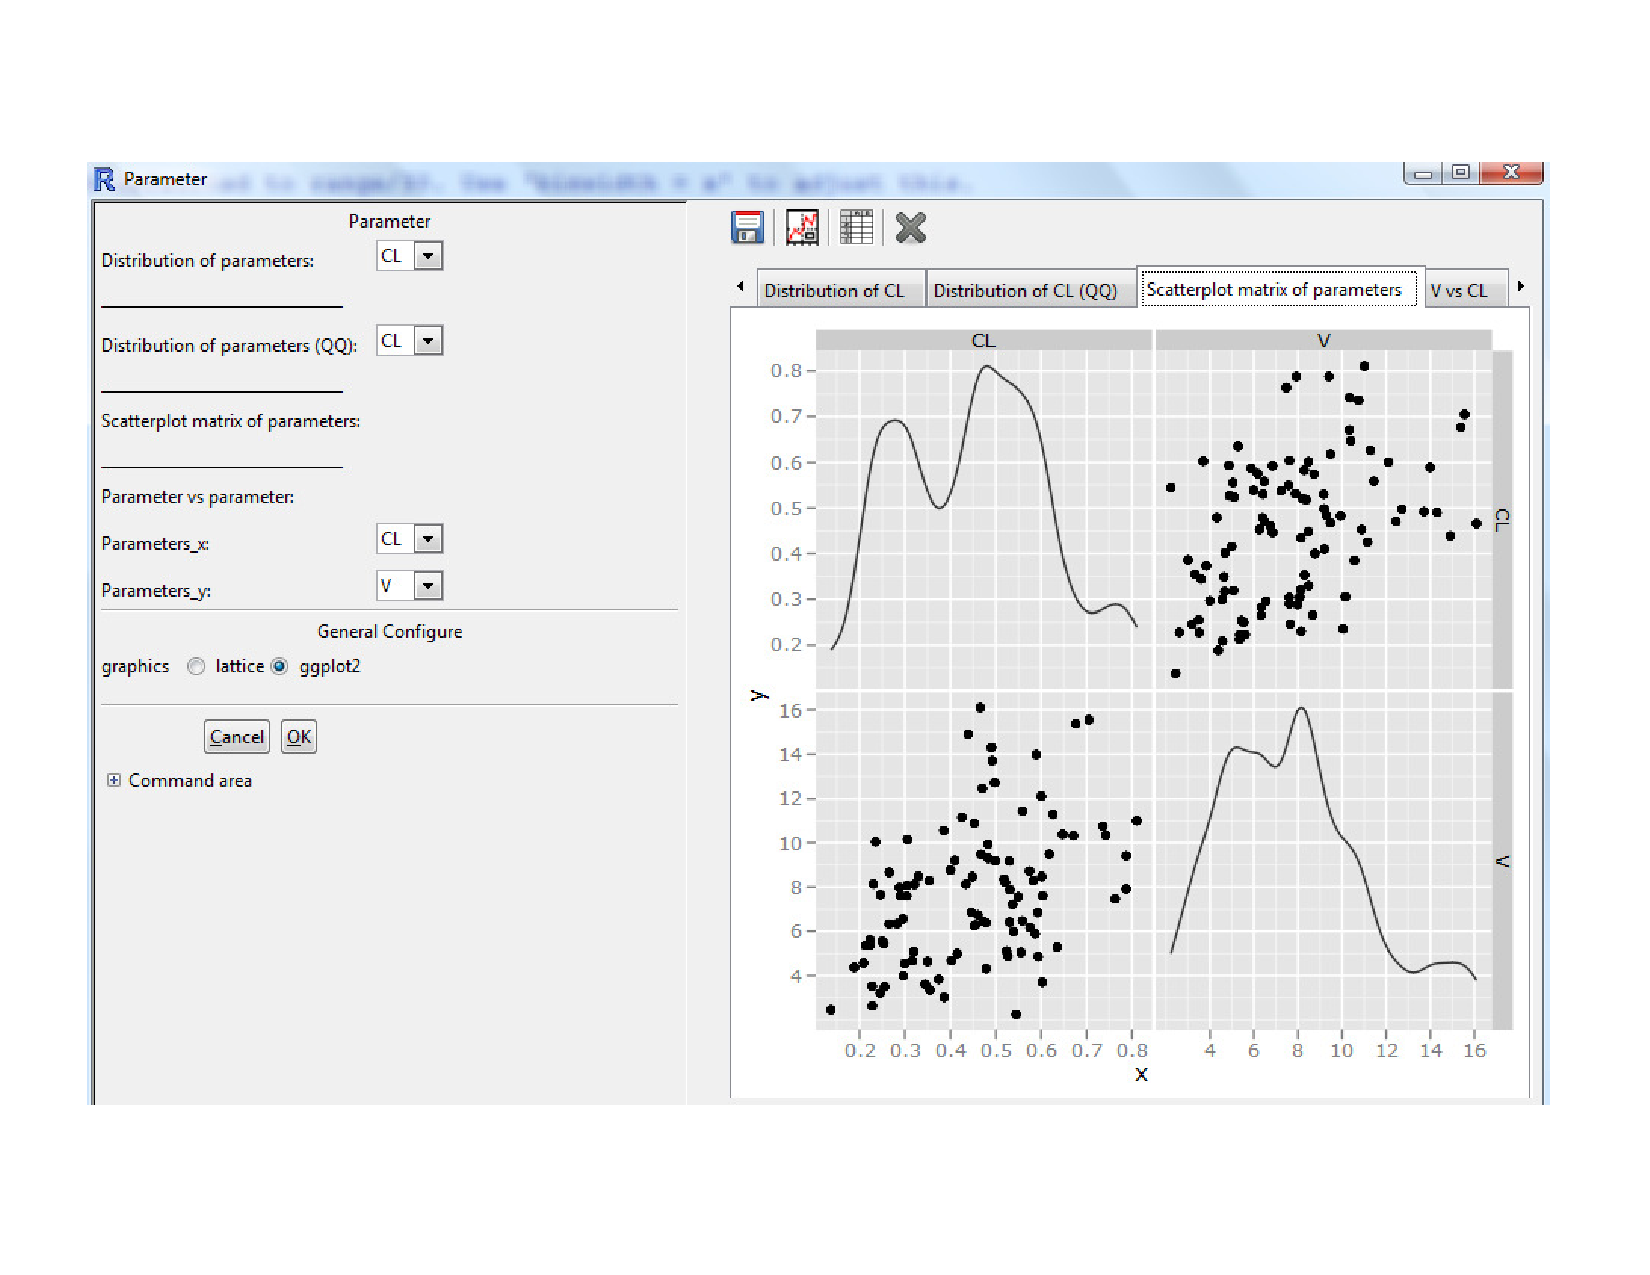
\includegraphics[scale=0.6]{pkmodel_para.pdf}
\caption{\textit{Parameters} in \textit{PK models}}
\label{pkmodel_para}
\end{figure}
%%%%%%%%%%%%%%
\subsubsection{Random effects}
The assumptions for random effects also need to be tested for distribution and correlation by histogram, scatter plots or a scatterplot matrix.
%%%%%%%%%%%%%%
\subsubsection{Structural model}
Structural model can be diagnosed by PRED versus concentration conditioned on time, IPRED versus concentration conditioned on time, WRES versus time, WRES versus PRED, PRED versus concentration conditioned on covariates, IPRED versus concentration conditioned on covariates.
%%%%%%%%%%%%%%
\subsubsection{Residual error model}
Two assumptions are related to this submodel: 1) homoscedastic variability; 2) symmetrically distributed residuals. To test these assumptions, we applied the following techniques: 1) histogram for distributions of WRES; 2) histogram for individual distribution of WRES; 3) scatterplot of $|$WRES$|$ versus PRED to check the shape of residual; 4) scatterplot of $|$WRES$|$ versus PRED conditioned on covariates to screen the covariate effects; 5) autocorrelation of WRES.
%%%%%%%%%%%%%%
\subsubsection{Covariate model}
Parameters, ETA and WRES are of great use to help screen proper covariates. We can utilize the following methods to check covariate models: 1) scatter plot for parameters versus covariates, ETAs versus covariates, WRES versus covariates; 2) scatterplot matrix of covariates.

%%%%%%%%%%%%%%%%%%%%%%%%%%%%%%%%%%%%%%%%%%%%%%%%%%%%%%%%%%%%%%%%%%%%%%%%%%%
\subsection{Model validation}
Resampling methods has been extensively employed in the model validation. Currently, bootstrap targets for confidence interval, case deletion diagnostics identify influential cases, and stochastic simulation is utilized to compare models.
PKgraph mainly focuses on case deletion diagnostics and bootstrap. 
\newline
\newline
It accepts two kinds of model validation data: 1) results from PsN; 2) results from multiple NONMEM runs. For the first type of data, PsN has the following functions: bootstrap, case deletion and stochastic simulation. PKgraph provides the graphic ability to visualize the final results from PsN. For the second type of data, PKgraph can handle multiple NONMEM run folders and extract useful information to visualize. \newline
\newline
\newline
It provides the following functions (Figure~\ref{modelv}),
\begin{itemize}
	\item \textit{Influence analysis summary (PsN)}: analyze PsN \textit{cdd} results.
	\item \textit{Visualization for influence analysis}: apply parallel coordinate plots and multidimensional scaling to visualize data from case deletion diagnostics (multiple NONMEM runs).
	\item \textit{Bootstrap summary (PsN)}: analyze PsN \textit{boot} results.
	\item \textit{Visualization for bootstrap}: visualize data from bootstrap (multiple NONMEM runs).
\end{itemize}
\begin{figure}[h!tb] \centering
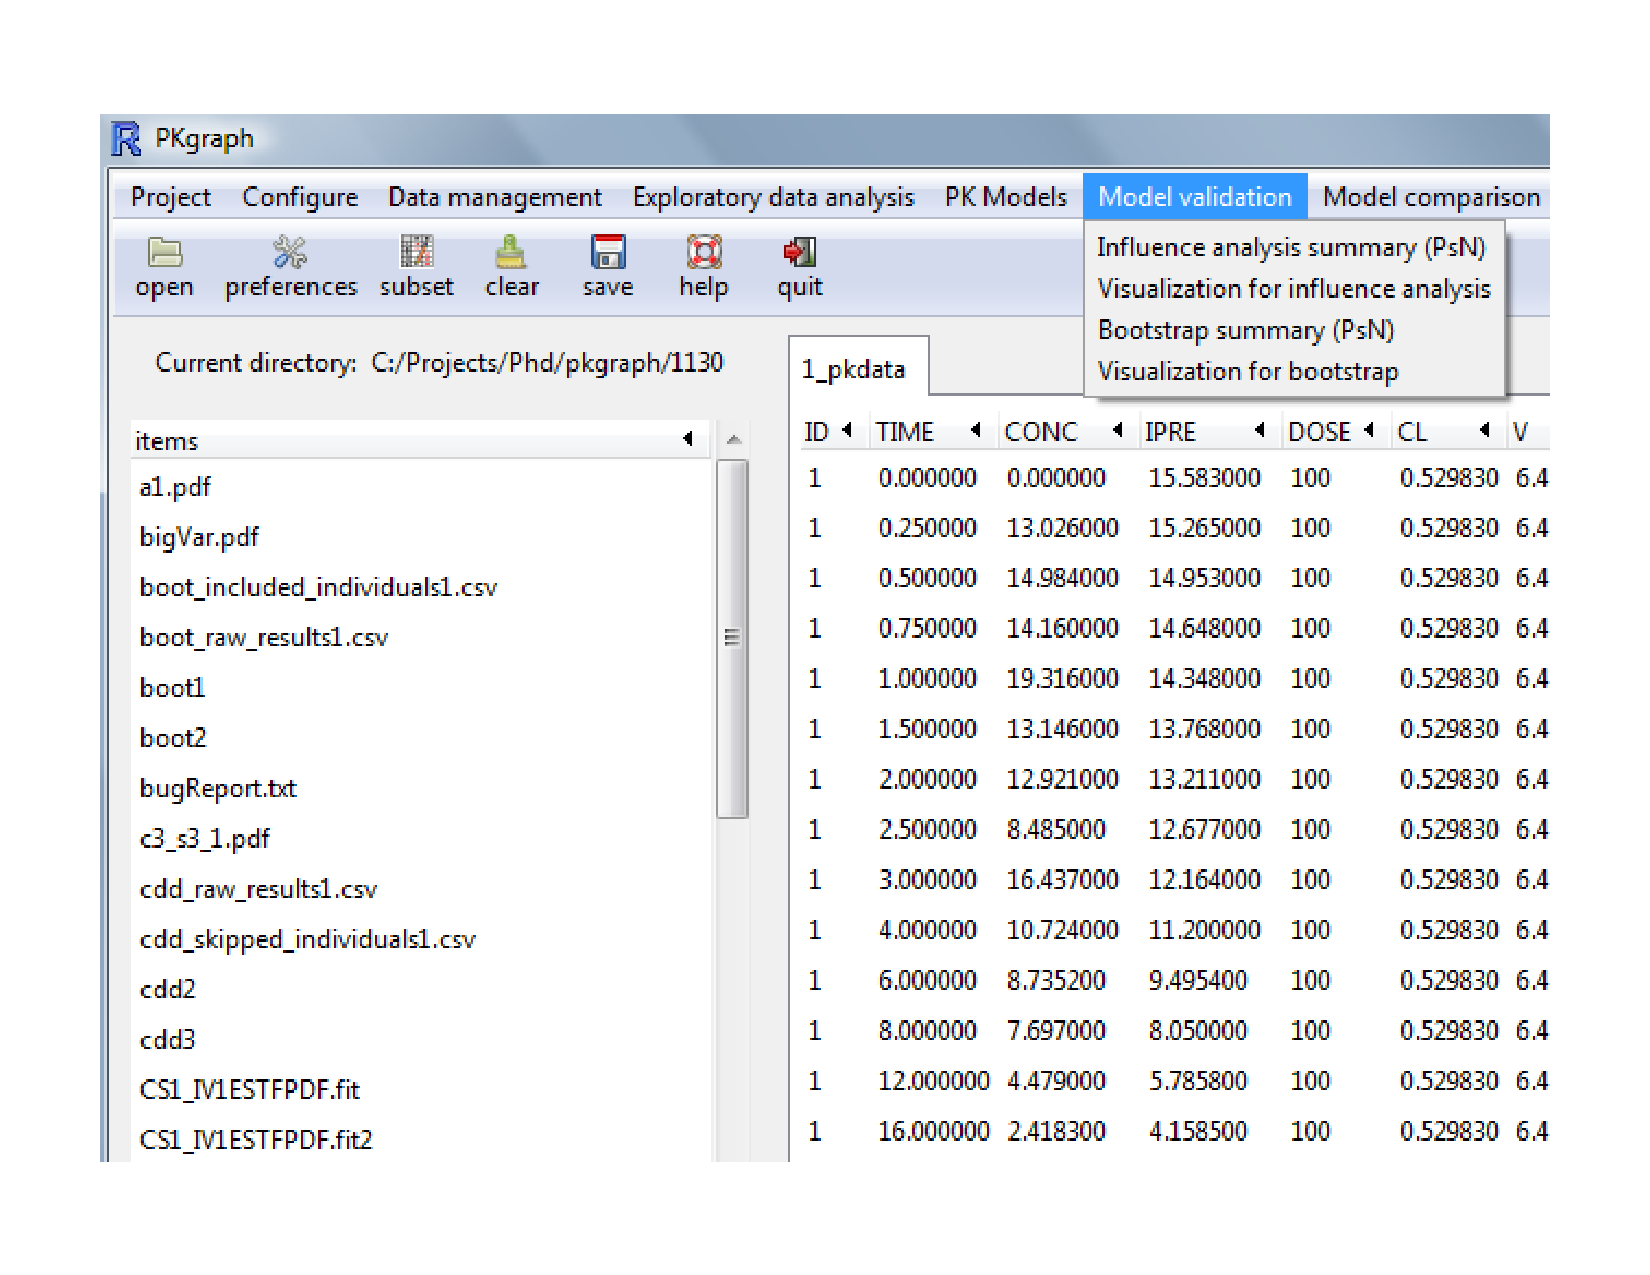
\includegraphics[scale=0.6]{modelv.pdf}
\caption{Menu items in \textit{Model validation}}
\label{modelv}
\end{figure}
%%%%%%%%%%%%%%%
\subsubsection{Influence analysis summary (PsN)}
This function is specifically for PsN \textit{cdd} results (Figure~\ref{infPsN}). It takes two result files from PsN: \textit{raw\_results1.csv} and \textit{skipped\_individuals1.csv}, and generates a scatter plot for cov.raito versus cov.score.
\begin{figure}[h!tb] \centering
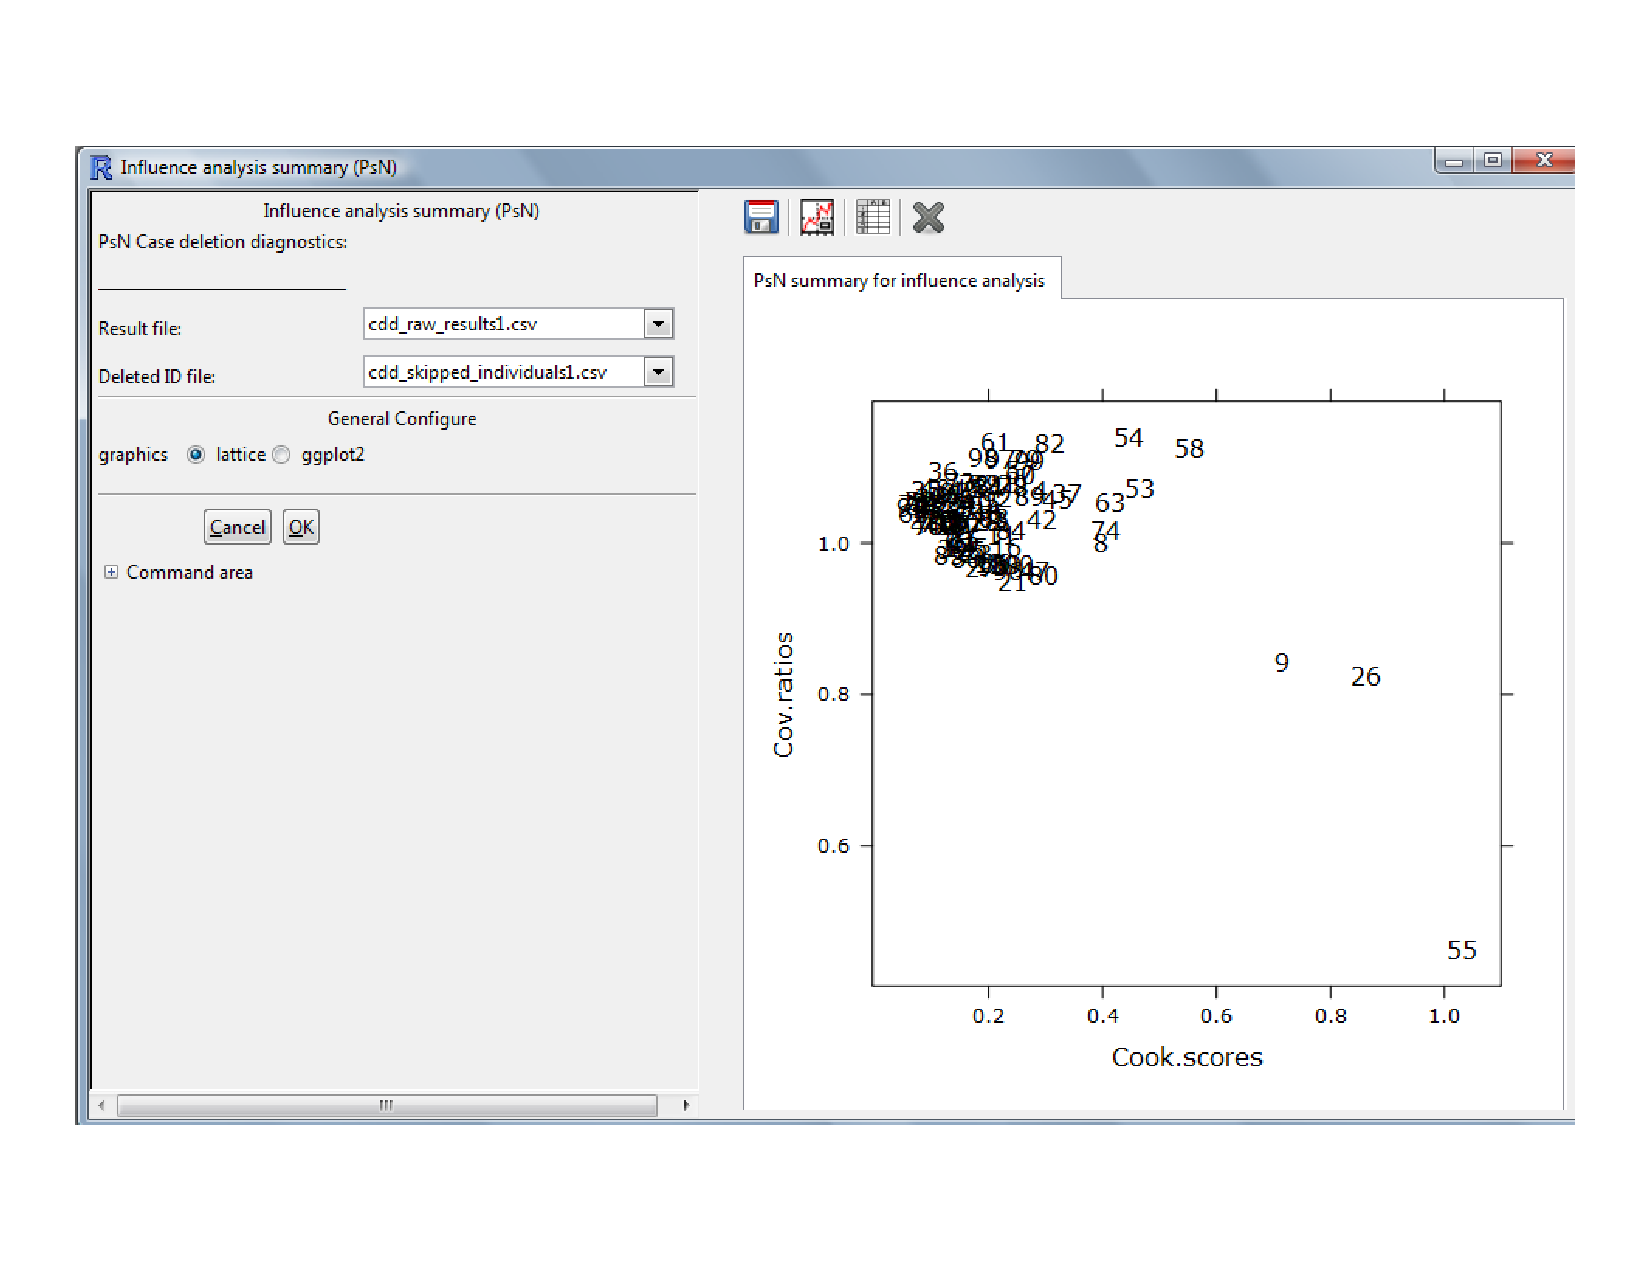
\includegraphics[scale=0.6]{infPsN.pdf}
\caption{Influence analysis summary (PsN)}
\label{infPsN}
\end{figure}
%%%%%%%%%%%%%%
\subsubsection{Visualization for influence analysis}
This function is to visualize data from case deletion diagnostics (multiple NONMEM runs). Let's use multiple NONMEM run form PsN directly (Figure~\ref{infCddData}), and find file directory for these runs. Then we can select parameters as shown in Figure~\ref{infCddPara}.  These parameters include:
\begin{itemize}
	\item \textit{Target directory path}: the path for multiple NONMEM runs. It is a required parameter.
	\item \textit{Simulation folder pattern}: the common folder name for multiple NONMEM runs. For this example, it is \textit{NM\_run}. It is a required parameter.
	\item \textit{NONMEM result file name}: the file name for NONEM fitted result. In each NONMEM run, there should be a file with this name. It is required parameter.	
	\item \textit{Patient ID}: the ID for each subject. It is a required parameter.
	\item \textit{Plot variable}: the variable you use to detect difference among patients. For this example, we choose \textit{CL}. It is a required parameter.
\end{itemize}
\begin{figure}[h!tb] \centering
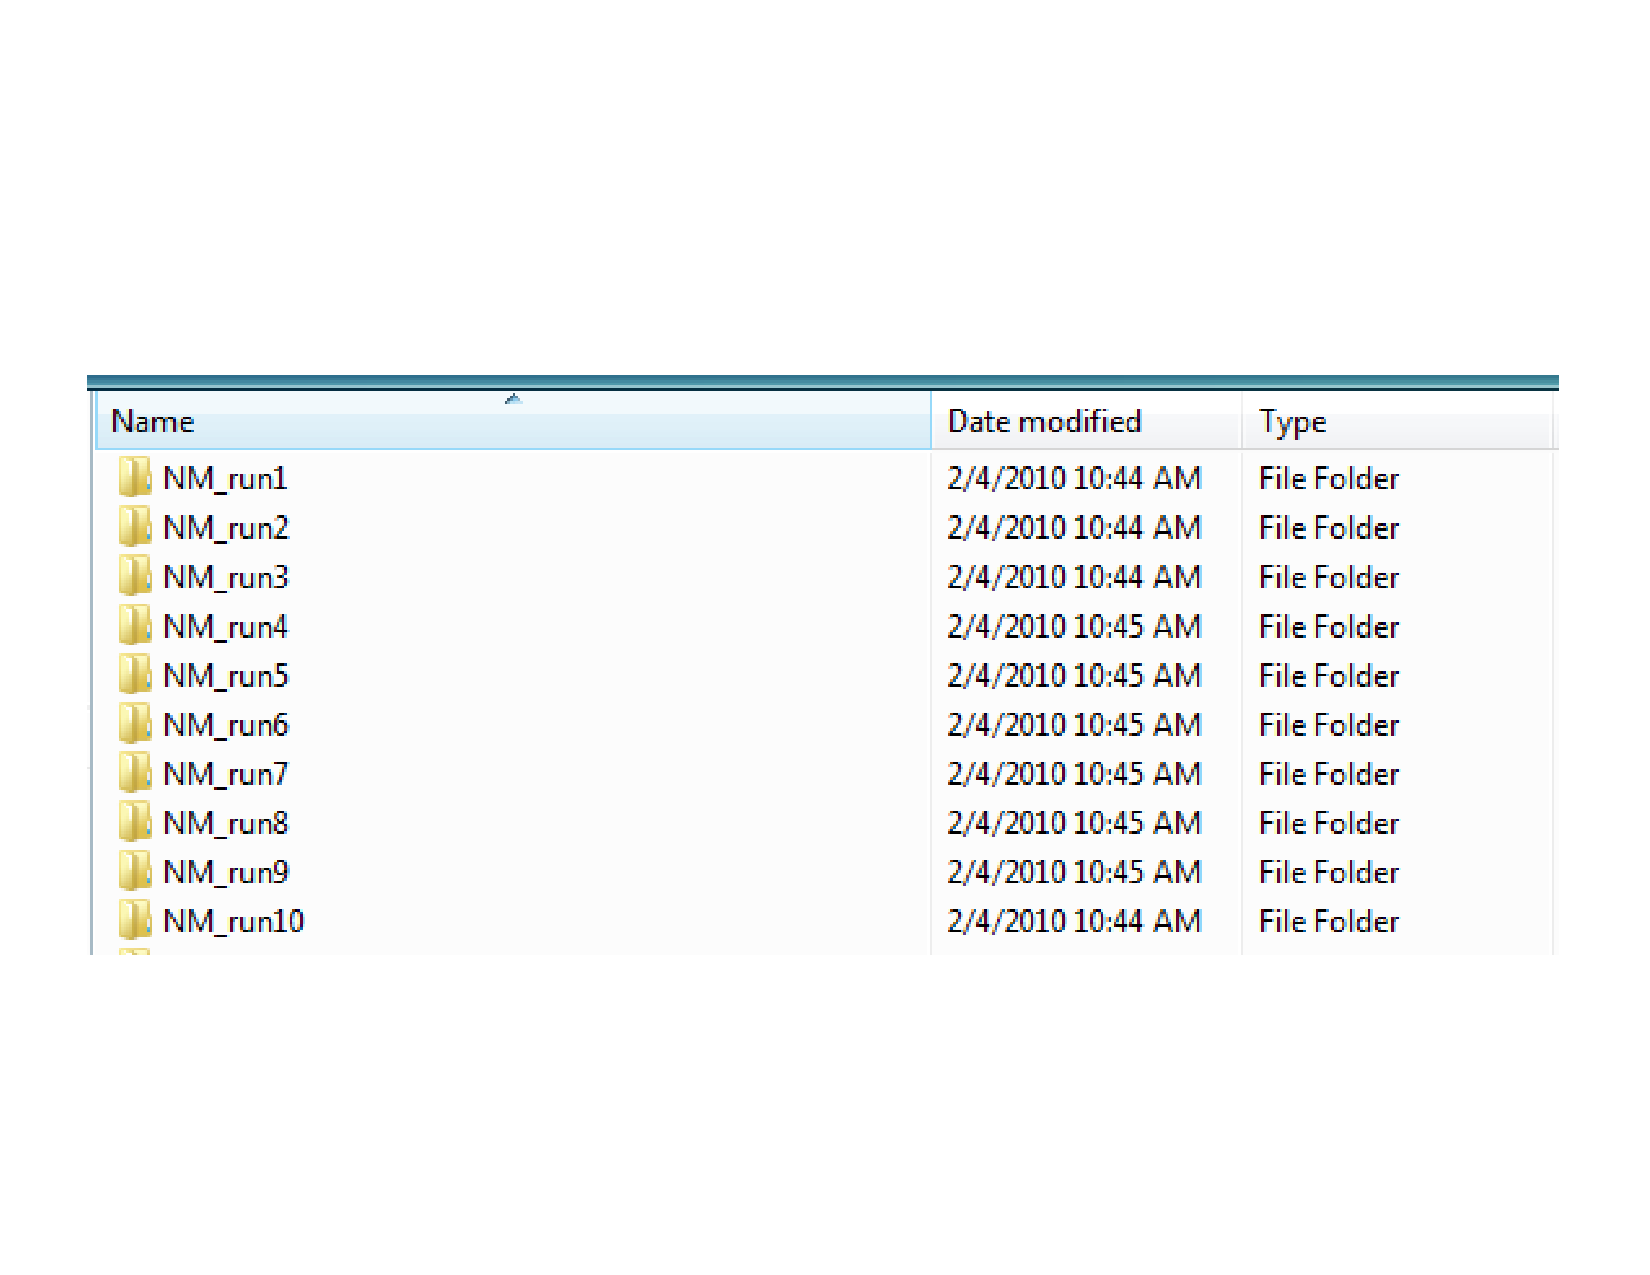
\includegraphics[scale=0.6]{infCddData.pdf}
\caption{Multiple NONMEM runs for case deletion diagnostics}
\label{infCddData}
\end{figure}
\begin{figure}[h!tb] \centering
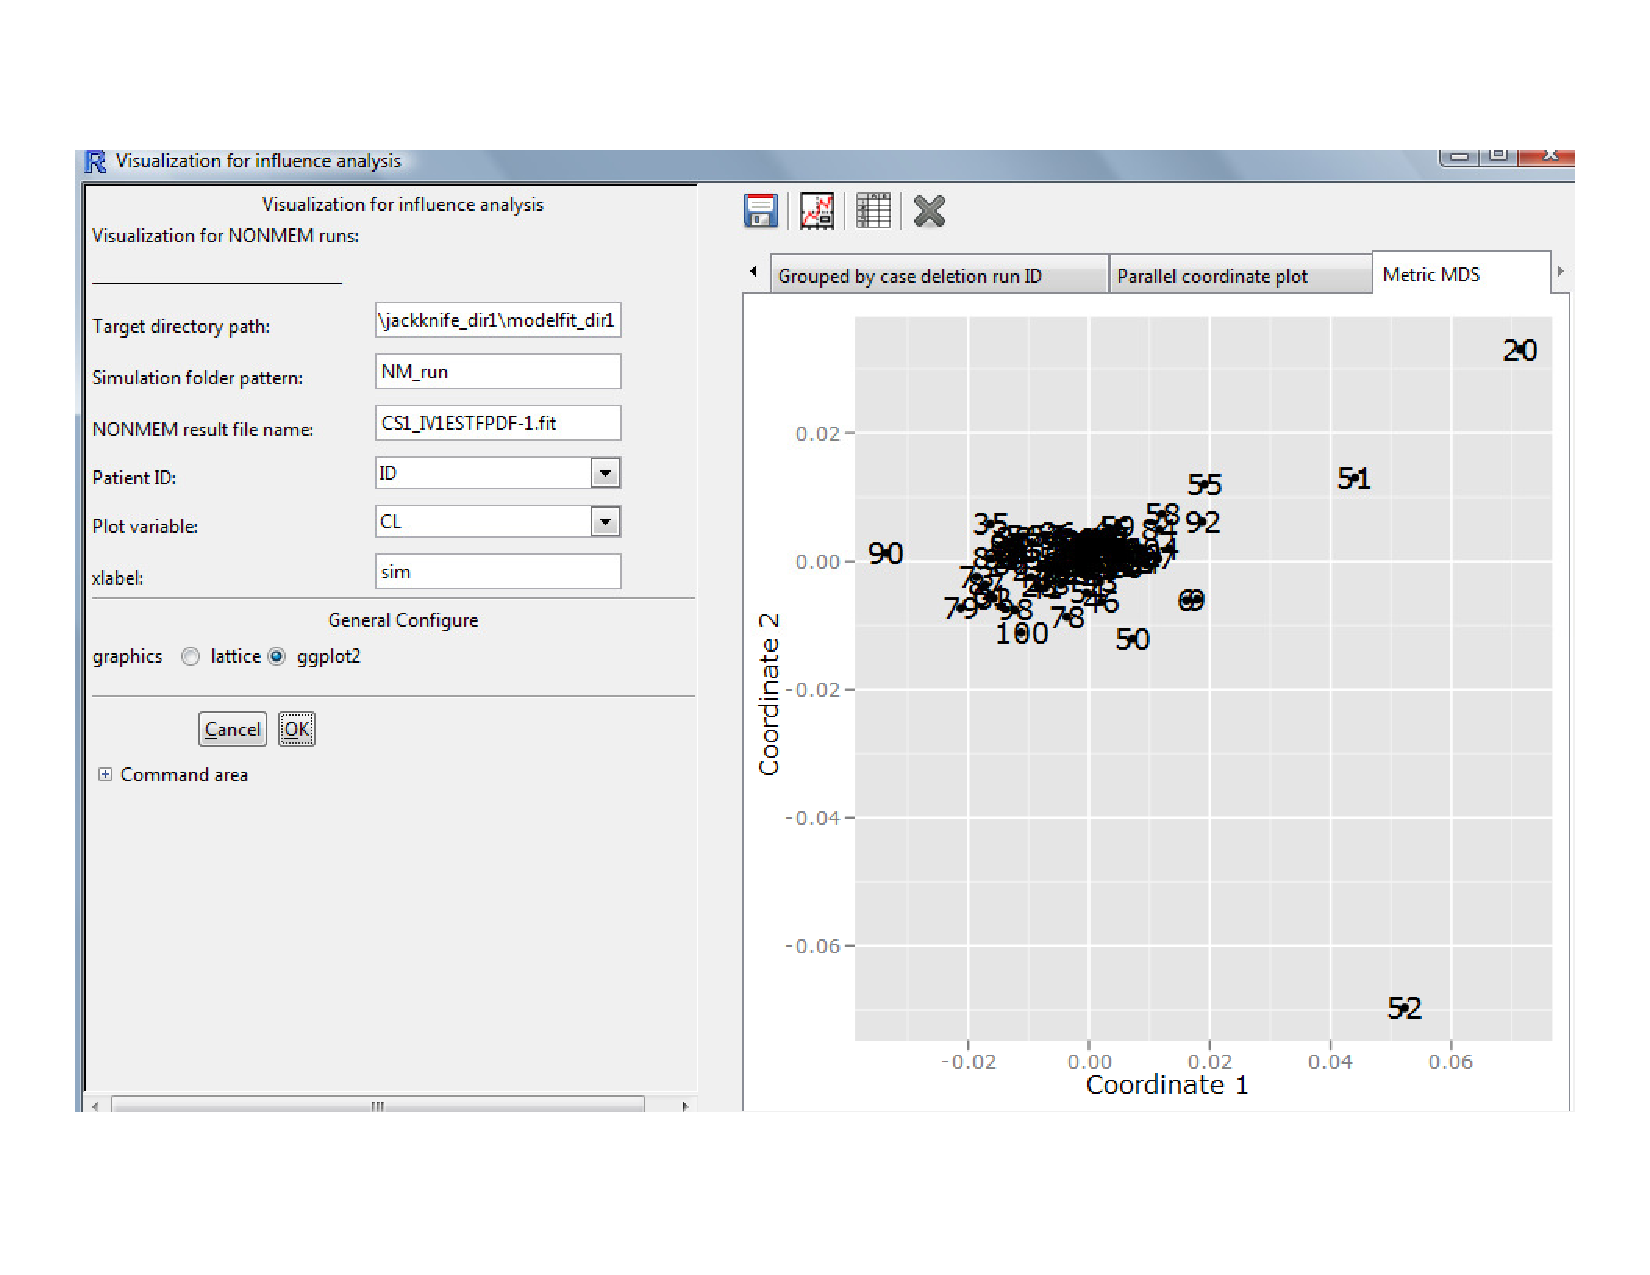
\includegraphics[scale=0.6]{infCddPara.pdf}
\caption{Parameters and results for case deletion diagnostics}
\label{infCddPara}
\end{figure}
%%%%%%%%%%%%%%%%%%%%%%
\subsubsection{Bootstrap summary (PsN)}
This function is specifically for PsN \textit{boot} results (Figure~\ref{bootPsN}). It takes two result files from PsN: \textit{raw\_results1.csv} and \textit{included\_individuals1.csv}, and generates related plots.
\begin{figure}[h!tb] \centering
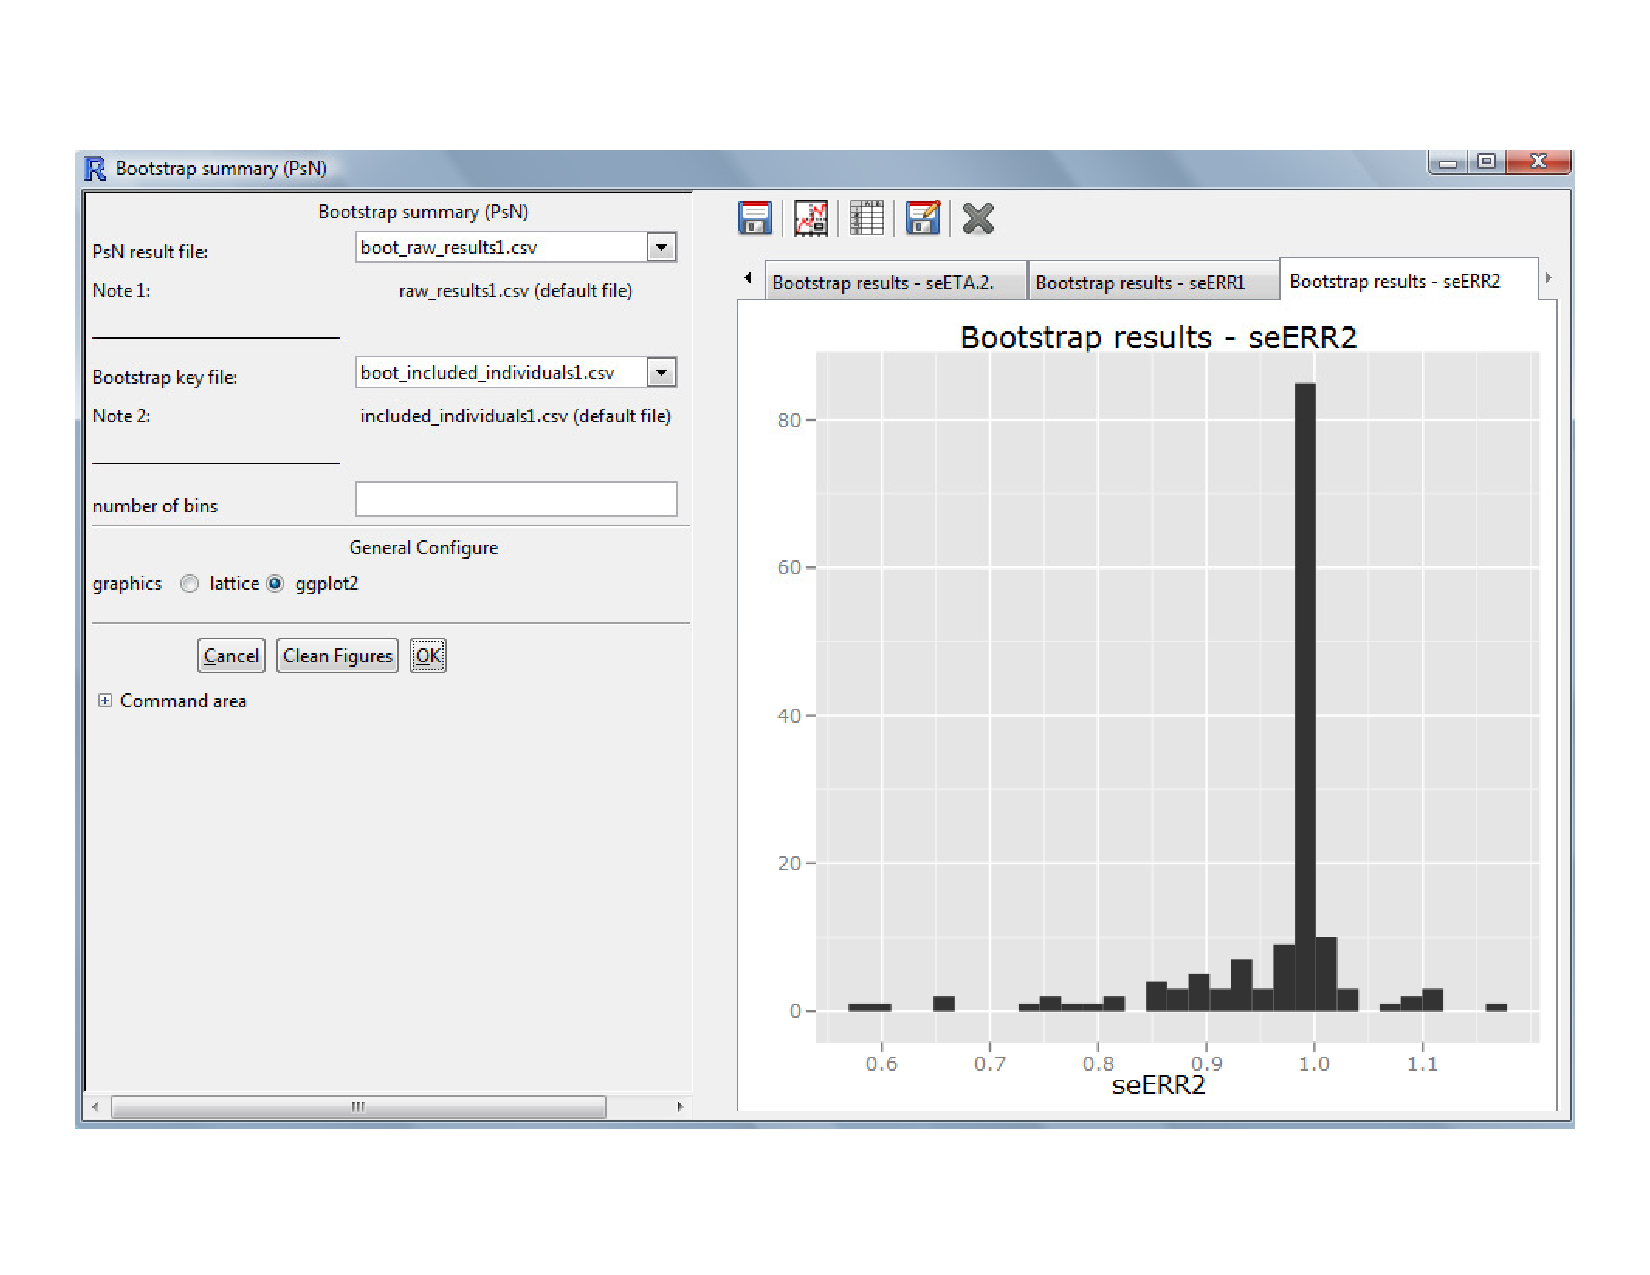
\includegraphics[scale=0.6]{bootPsN.pdf}
\caption{Bootstrap summary (PsN)}
\label{bootPsN}
\end{figure}
%%%%%%%%%%%%%%%%%%%
\subsubsection{Visualization for bootstrap}
This function is to visualize data from boostrap (multiple NONMEM runs). Let's use multiple NONMEM run form PsN (Figure~\ref{bootData}), and find file directory for these runs. Then we can select parameters as shown in Figure~\ref{bootPara}.  These parameters include:
\begin{itemize}
	\item \textit{Target directory path}: the path for multiple NONMEM runs. It is a required parameter.
	\item \textit{Bootstrap folder pattern}: the common name style for multiple NONMEM runs. For this example, it is \textit{NM\_run}. It is a required parameter.
	\item \textit{NONMEM result file name}: the fit result for each NONMEM run. In this example, it is \textit{CS1\_IV1ESTFPDF-1.fit }. It is a required parameter.
	\item \textit{Bootstrap key table path}: the path for bootstrap key file, which is file describing the sampling schema for patient IDs. It is a required parameter.
	\item \textit{Bootstrap key table name}: The file describes the sampling schema for patient IDs In this example, it is \textit{included\_individuals1.csv}. It is a required parameter.
	\item \textit{Patient ID}: the ID for each subject. It is a required parameter.
	\item \textit{Plot variable}: the variable you use to detect difference among patients. For this example, we choose \textit{CL}. It is a required parameter.
	\item \textit{xlabel}: the name label for each NONMEM run. It is optional.
\end{itemize}
\begin{figure}[h!tb] \centering
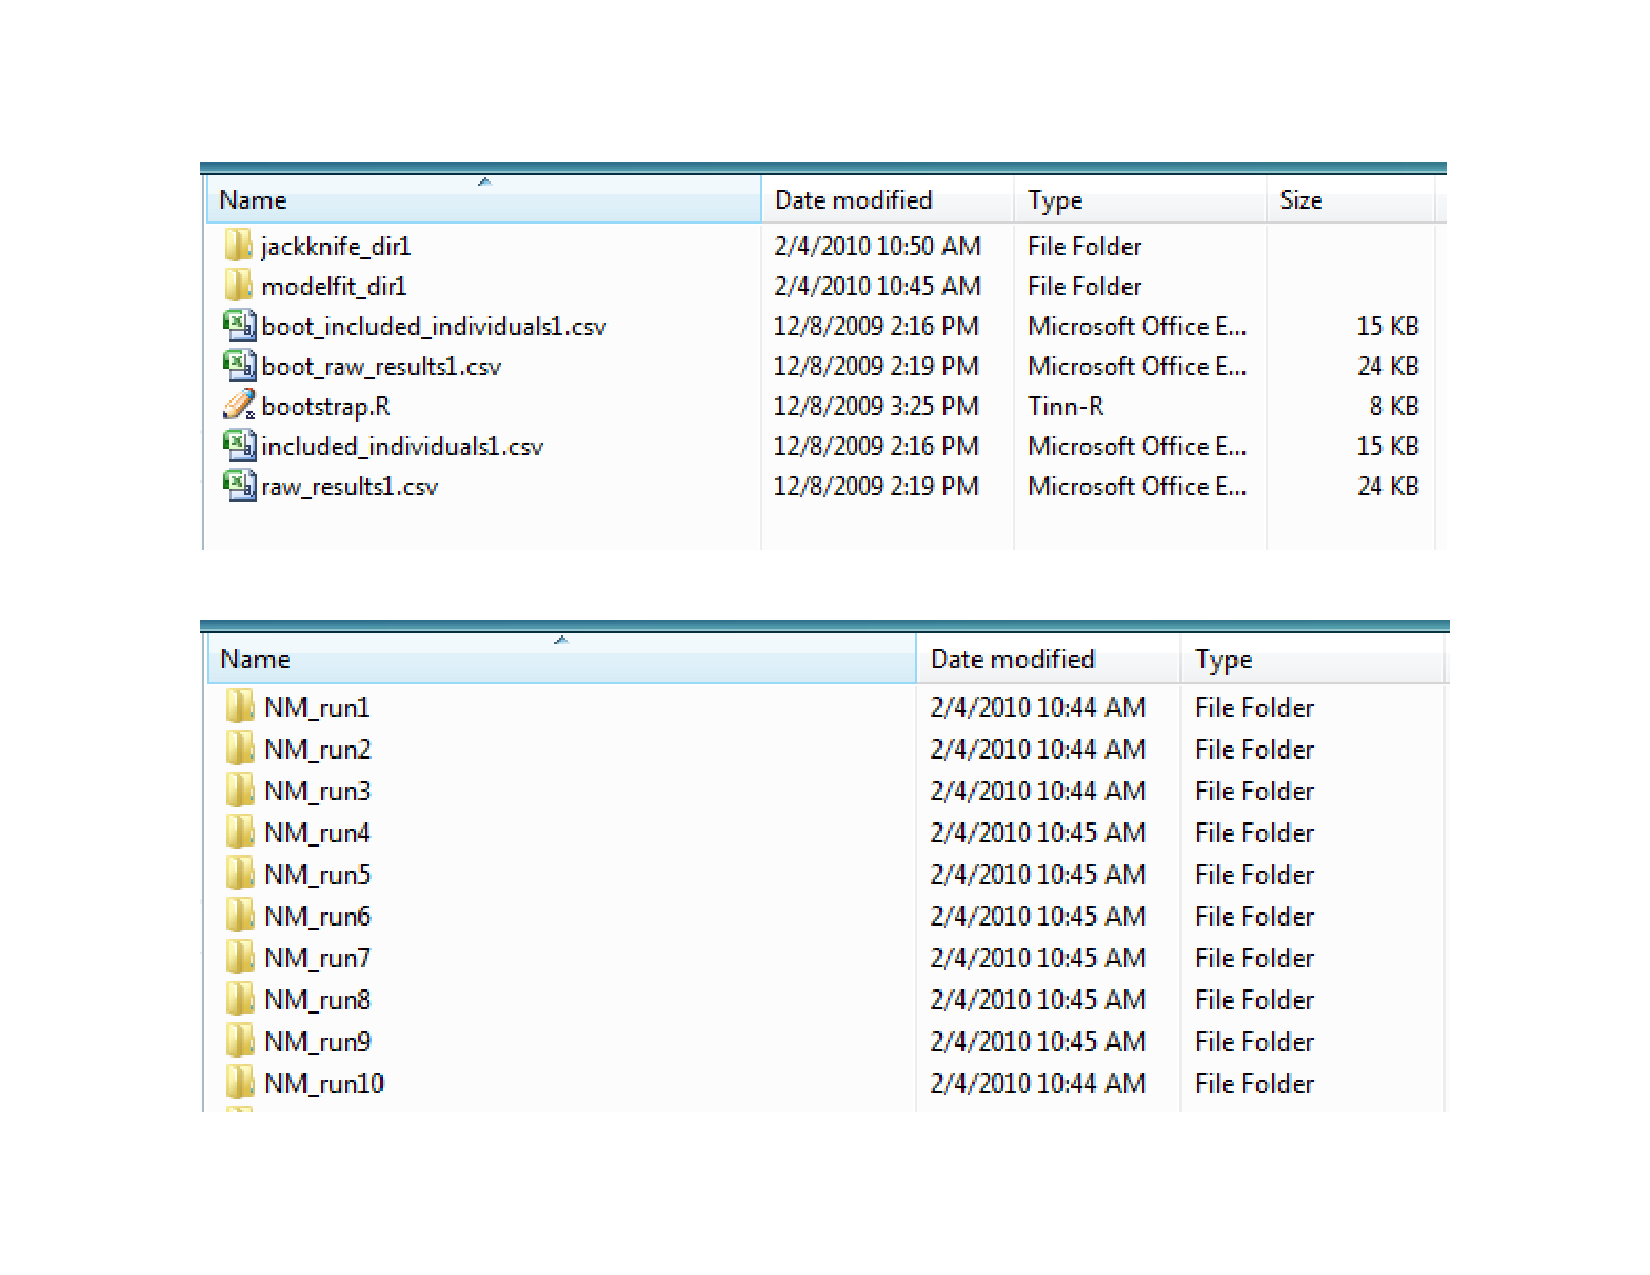
\includegraphics[scale=0.6]{bootData.pdf}
\caption{Multiple NONMEM runs for bootstrap}
\label{bootData}
\end{figure}
\begin{figure}[h!tb] \centering
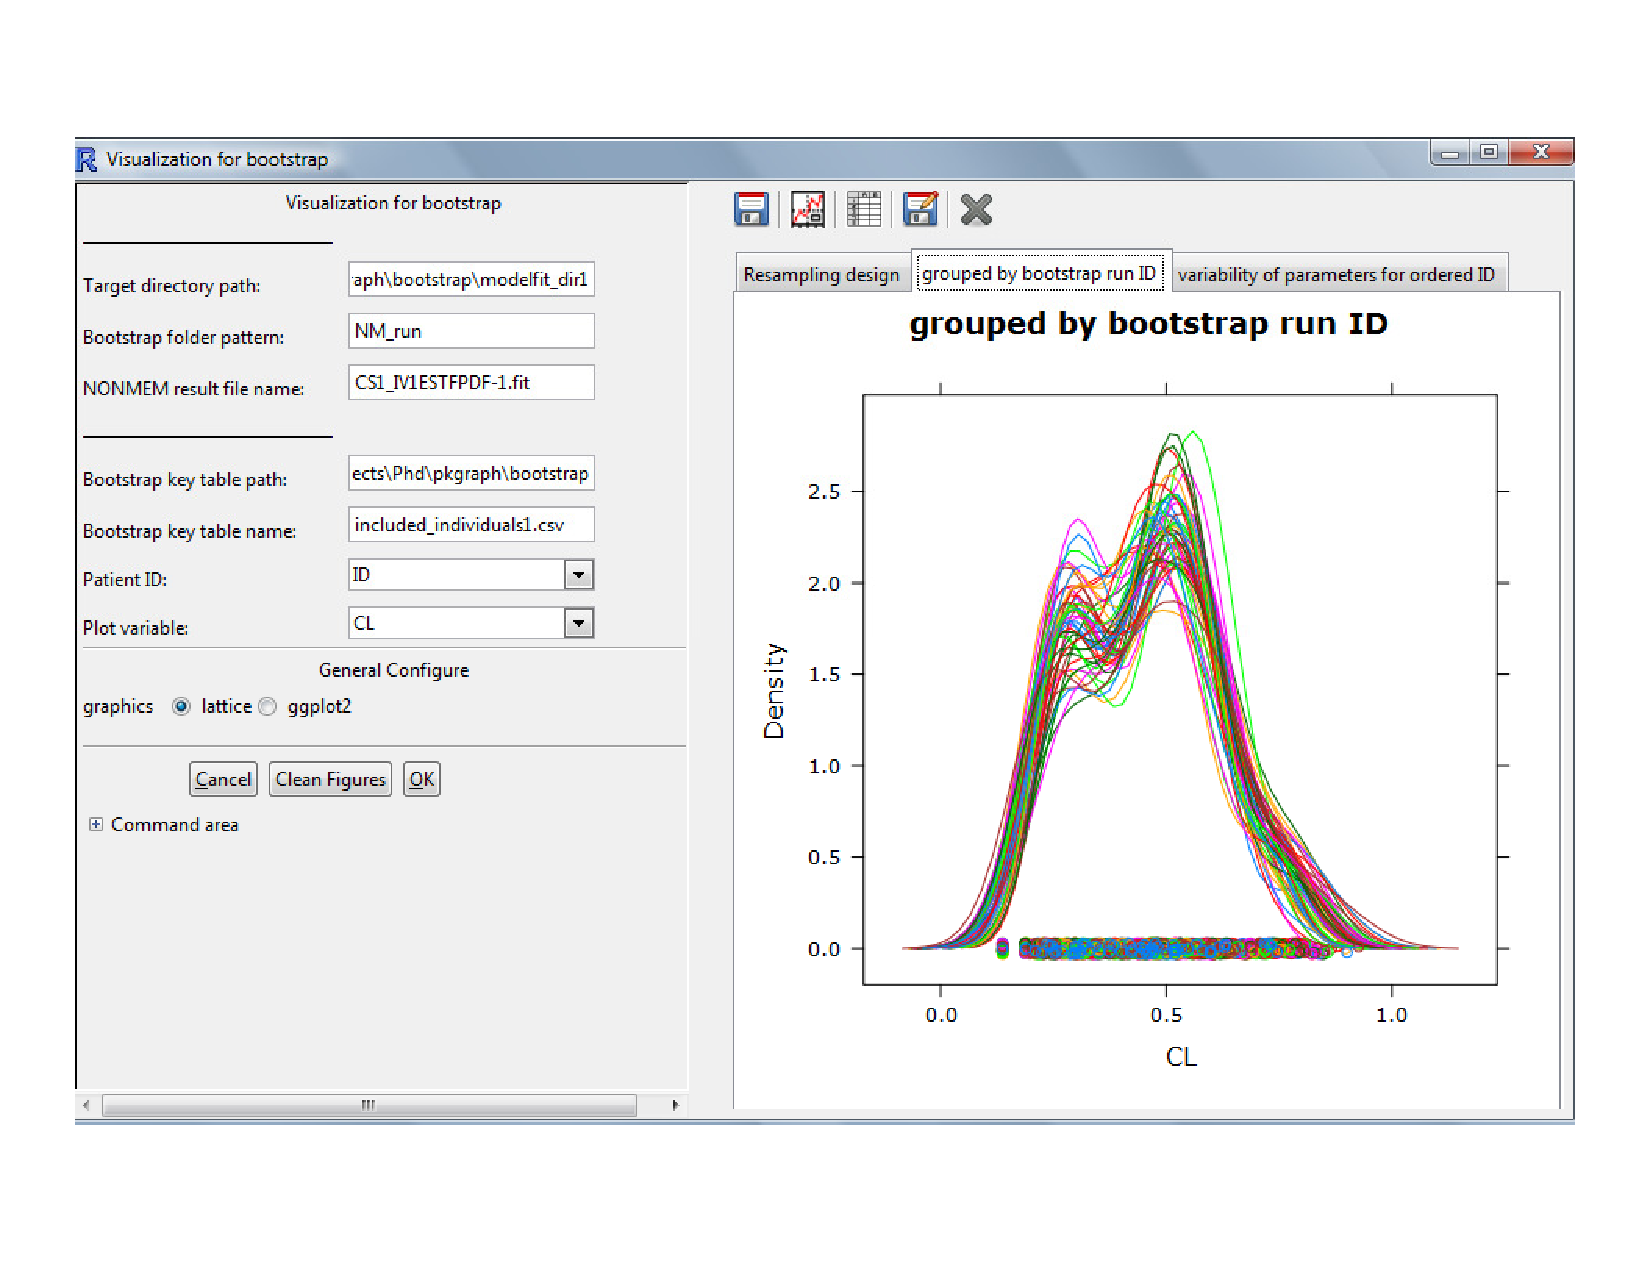
\includegraphics[scale=0.6]{bootPara.pdf}
\caption{Parameters and results for bootstrap visualization}
\label{bootPara}
\end{figure}
%%%%%%%%%%%%%%%%%%%%%%%%%%%%%%%%%%%%%%%%%%%%%%%%%%%%%%%%%%%%%%%%%%%%%%%
\subsection{Model comparison}
In this process, there are three main steps: 1) select datasets; 2) configure mapping; 3) comparison (Figure~\ref{modelc}). The first step is to select datasets for comparison. Currently the program only supports comparison of two models. Then users proceed to configure mapping by matching column names or variable names from two data sets. These matching variables are generally the variables from original data sets and they are not related to model fitting. For example, we have to match TIME, ID, CONC, WT, etc from original data, but not match those variables from model fit, such as ETA, RES, WRES, etc. When all parameters are set, the program offers three choices for comparison: ``histogram comparison'' (distribution comparison), ``scatter plot comparison'' and ``transform comparison''.\begin{figure}[h!tb] \centering
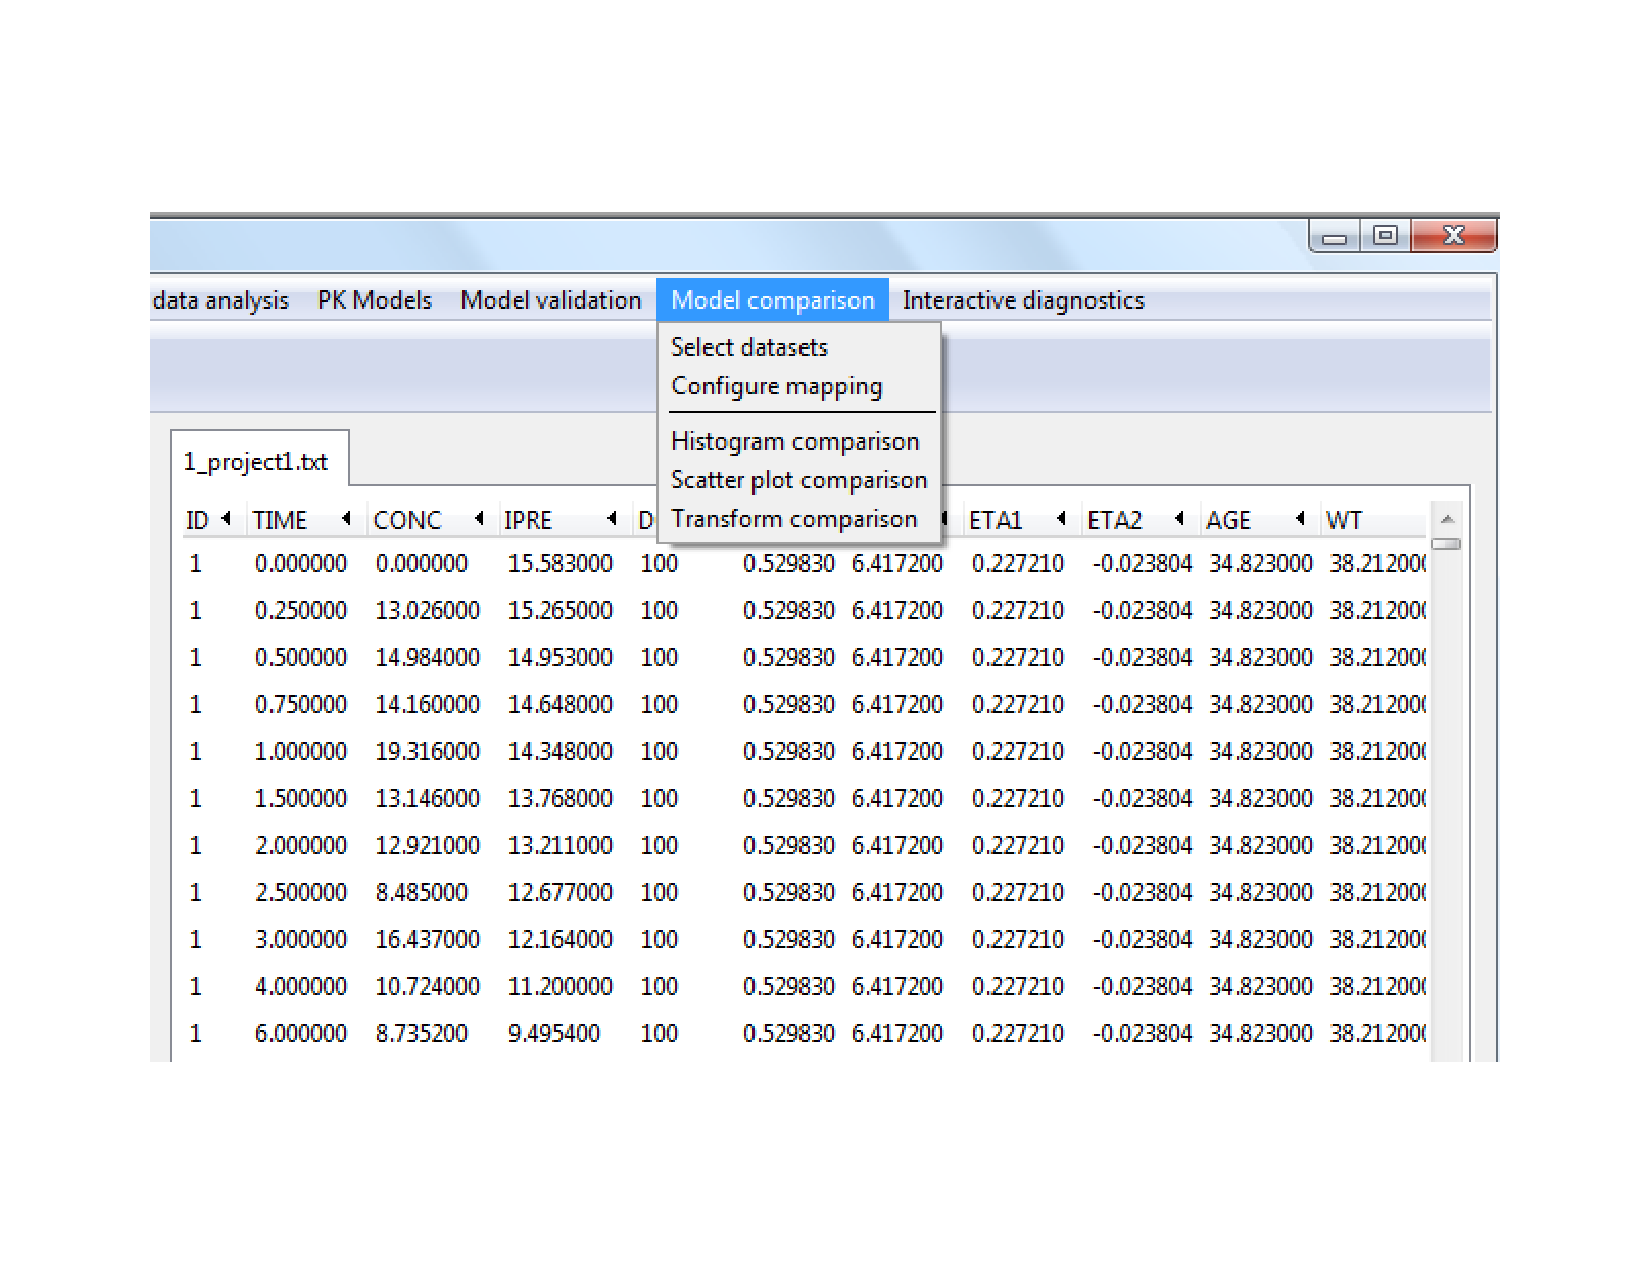
\includegraphics[scale=0.6]{modelc.pdf}
\caption{Menu items in \textit{Model comparison}}
\label{modelc}
\end{figure}
%%%%%%%%%%%
\subsubsection{Select datasets}
This function is to select datasets available in the PKgraph data area. Figure~\ref{modelcData} shows there are three data sets available, including fit result 2:  2\_CS1\_IV1ESTFPDF.fit (fit with additive error model) and fit result 3: 3\_ CS1\_IV1ESTFPDF.fit2 (proportional error model). In this example, we will compare these two models.
\begin{figure}[h!tb] \centering
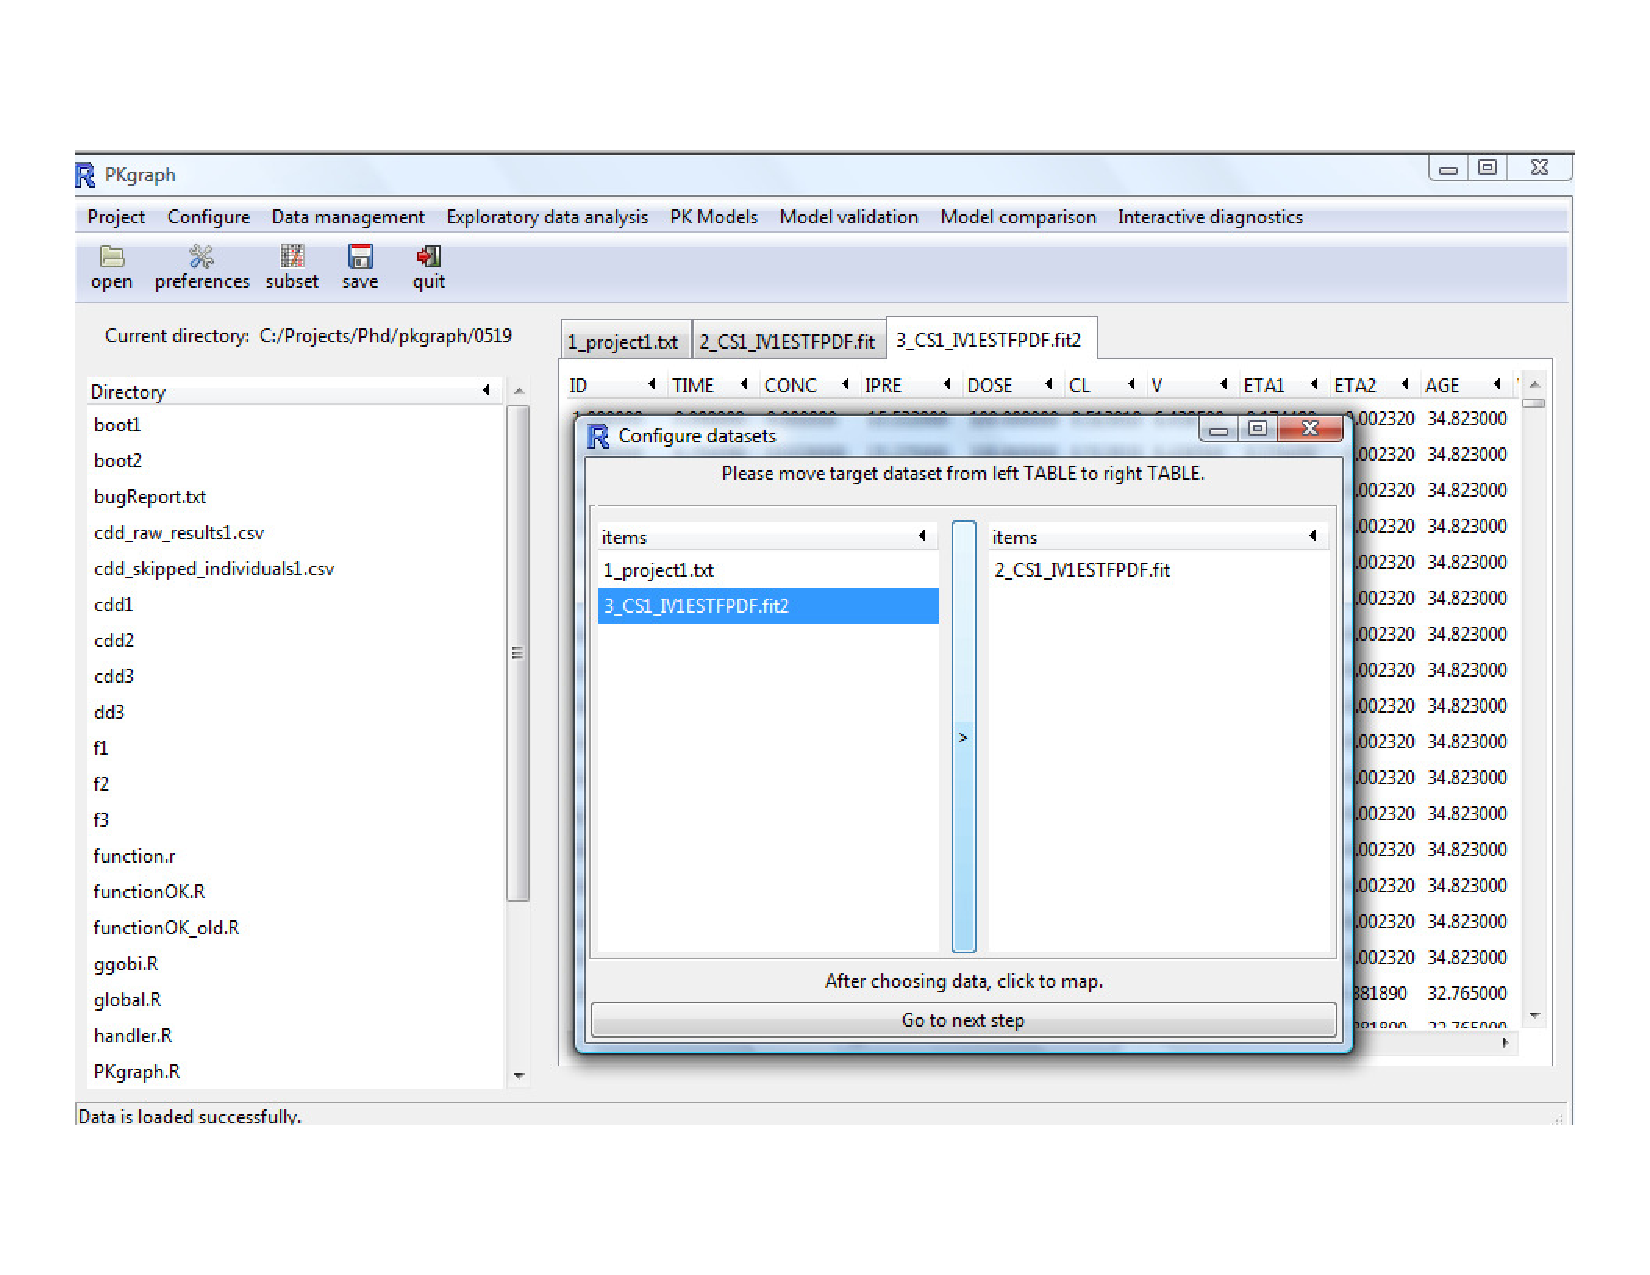
\includegraphics[scale=0.6]{modelcData.pdf}
\caption{\textit{Select datasets} in \textit{Model comparison}}
\label{modelcData}
\end{figure}
%%%%%%%%%%%%%%
\subsubsection{Configure mapping}
This step will join two fit results. As a result, users have to match the original data variables between two fit results. For example (Figure~\ref{modelcMap}),
\begin{itemize}
	\item \textit{Matching variables}: \textit{ID, Time, Concentration, WT, AGE}, etc must be matched in this step. These variables do not change with different models.
	\item \textit{Non-matching variables}: \textit{RES, PRED, WRES}, etc are fit results, and should NOT be matched. These variables change with different models.
\end{itemize}
After mapping, a new dataset joining two fit results will show in data area of main interface.
\begin{figure}[h!tb] \centering
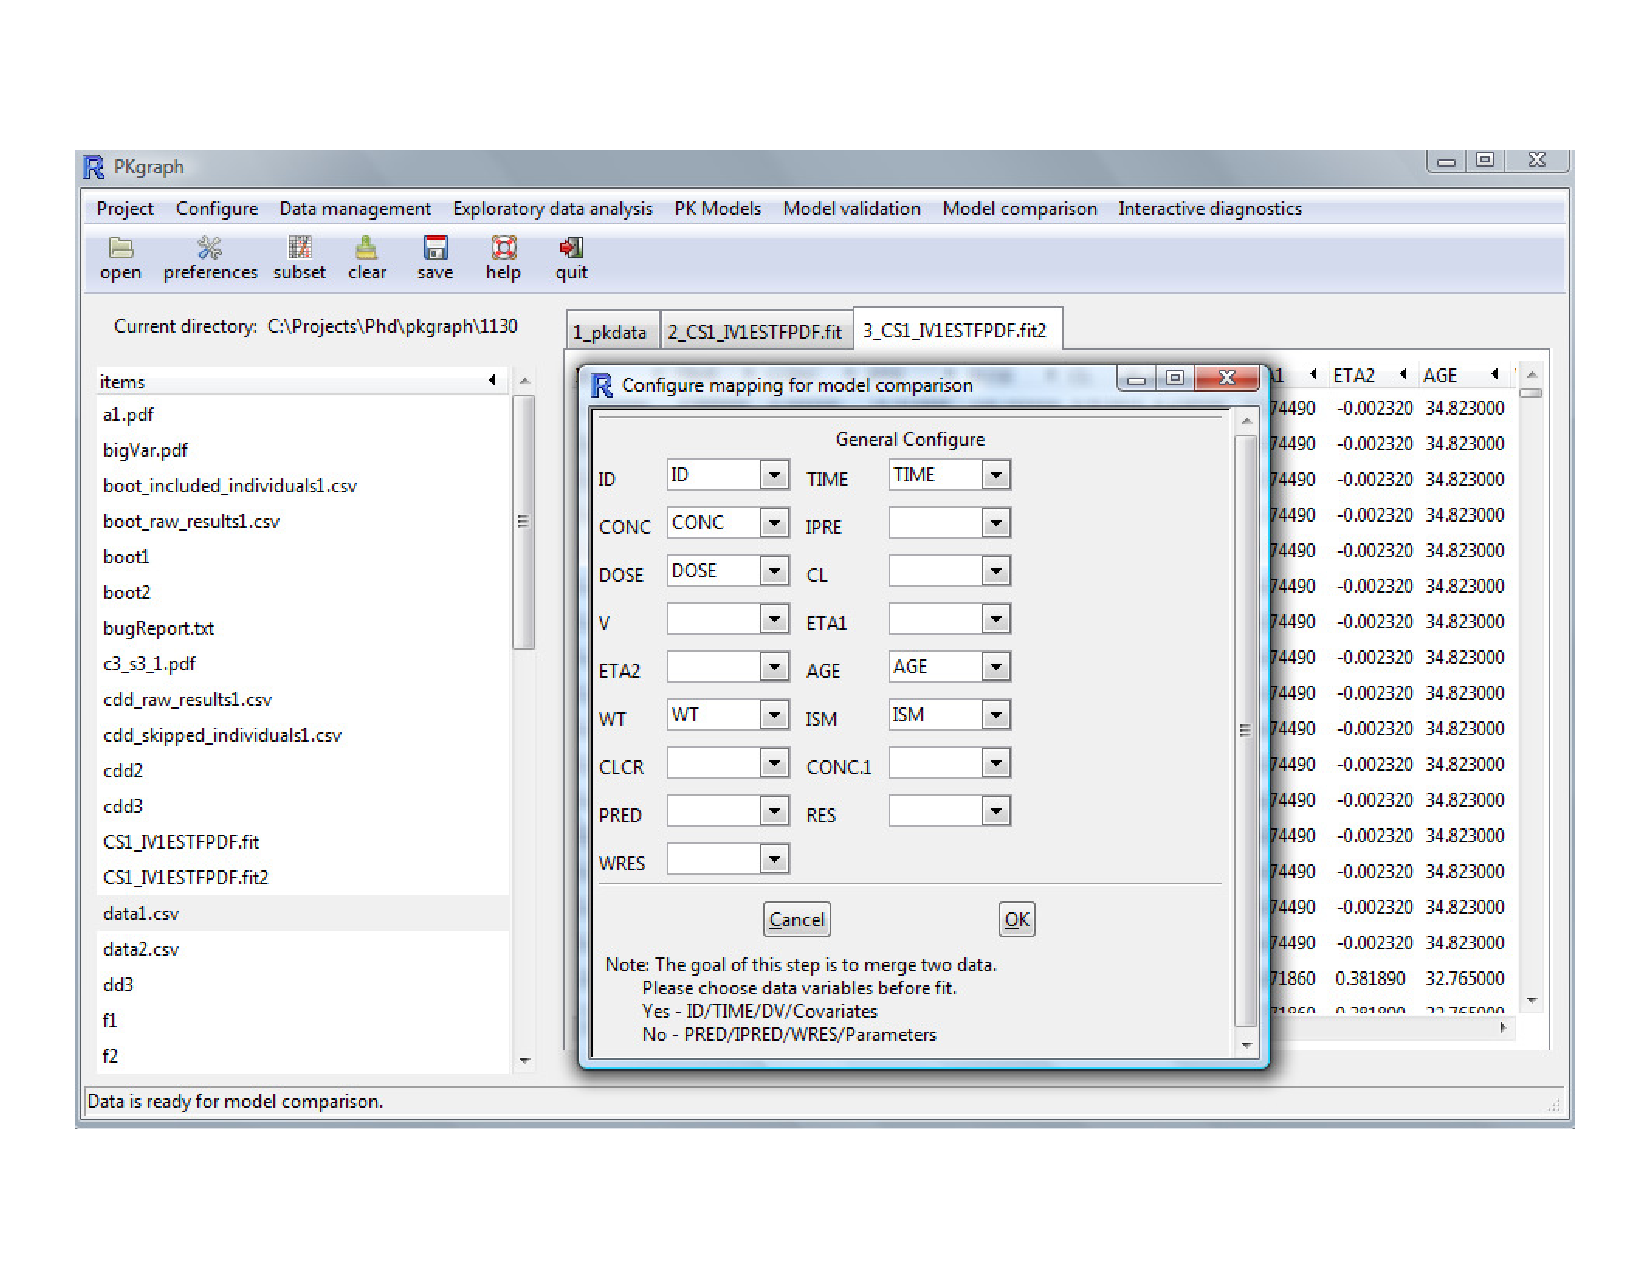
\includegraphics[scale=0.6]{modelcMap.pdf}
\caption{\textit{Configure mapping} in \textit{Model comparison}}
\label{modelcMap}
\end{figure}
%%%%%%%%%%%%%%%
\subsubsection{Comparison}
``histogram comparison'' enables to compare distributions of matching parameters from two models. ``scatter plot comparison''  provides an environment to compare matching parameters by scatter plot. ``transform comparison''  transforms data by ratio or log ratio in order to visualize the difference between variables from two models. All these models can be linked directly to ggobi for interactive diagnostics by clicking second button in the tool bar area on the top right panel.
\newline
\newline
All variable names for model 1 will have additional ``.x'' label, and all variable names for model 2 will have additional ``.y'' label.
\newline
\newline
Let us look at ``histogram comparison'' as one example. First, we need to make sure that current data set is ``4\_ModelComparison'' (Figure~\ref{modelcc1}); second, we click ``histogram comparison''. The result is shown in (Figure~\ref{modelcc2}) for comparing \textit{CL}.\begin{figure}[h!tb] \centering
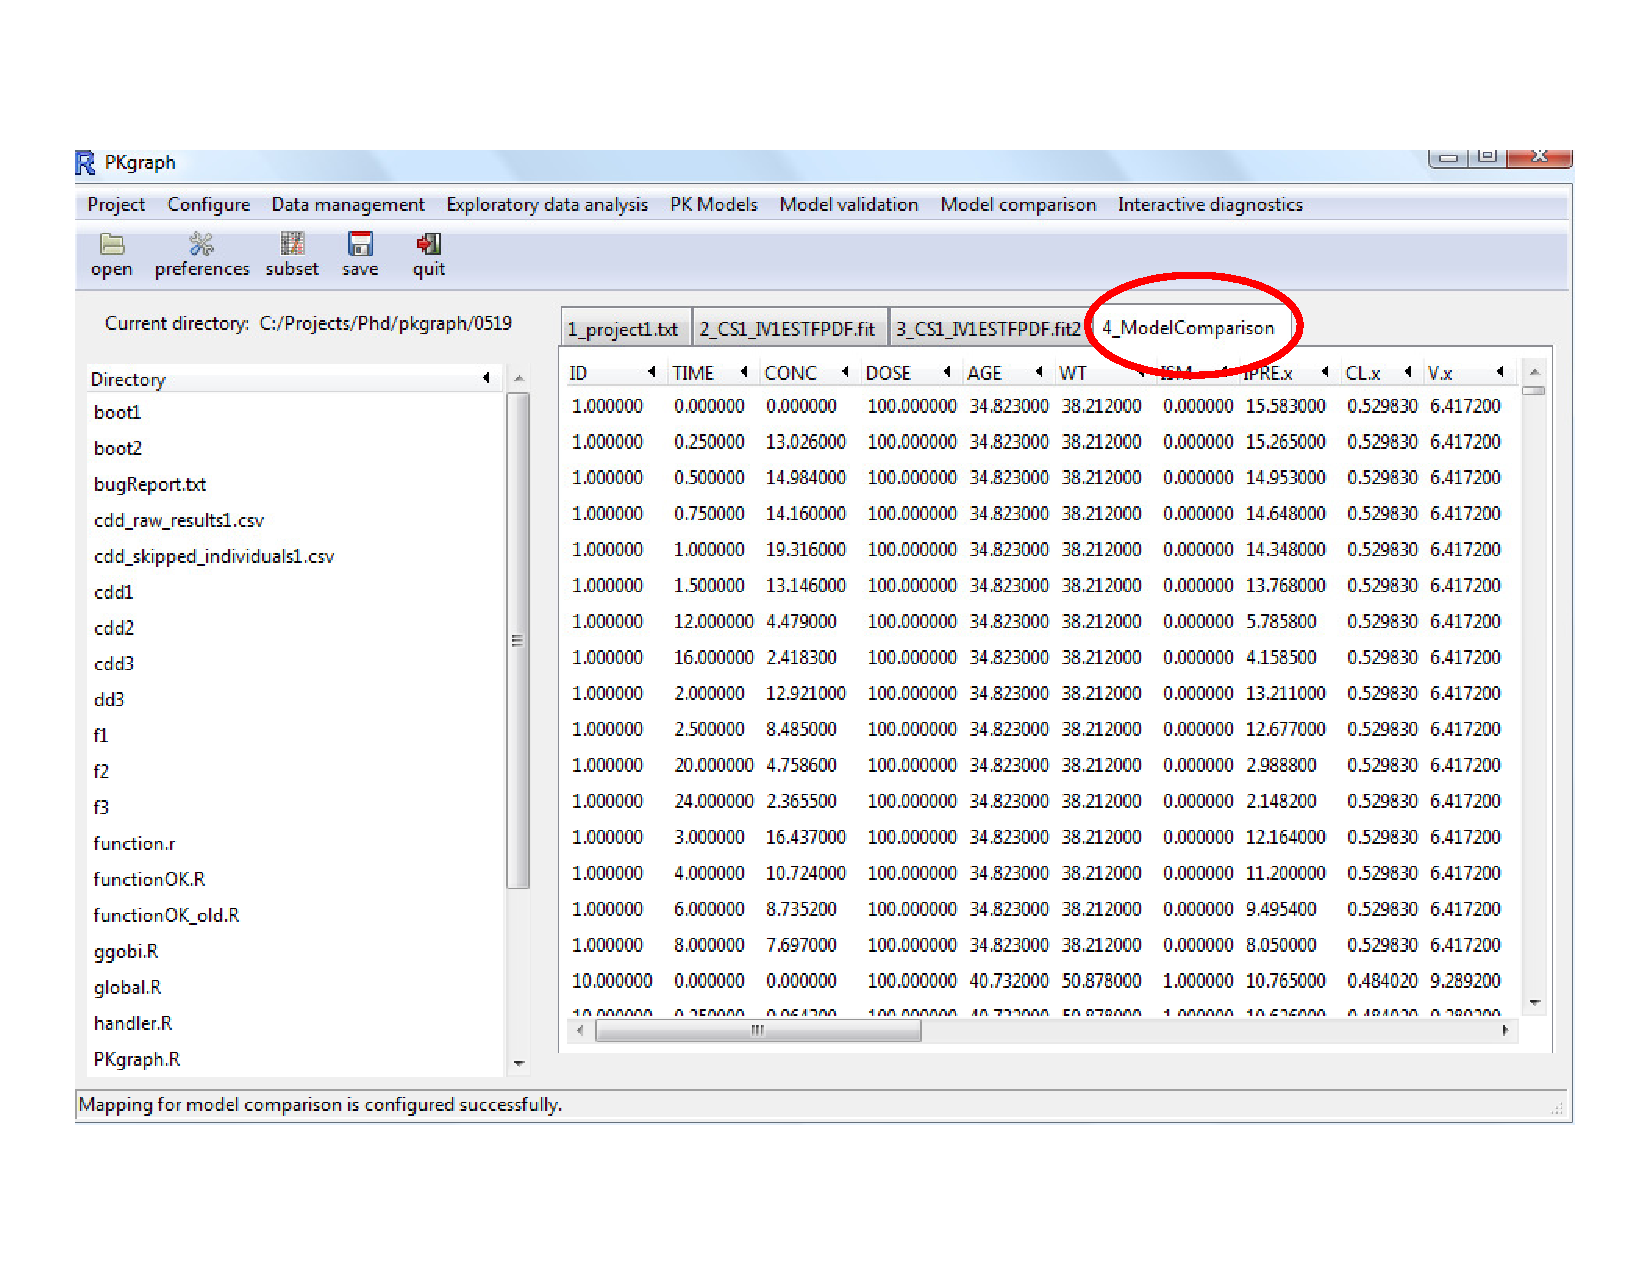
\includegraphics[scale=0.6]{modelcc1.pdf}
\caption{Current data set for \textit{Model comparison}}
\label{modelcc1}
\end{figure}
\begin{figure}[h!tb] \centering
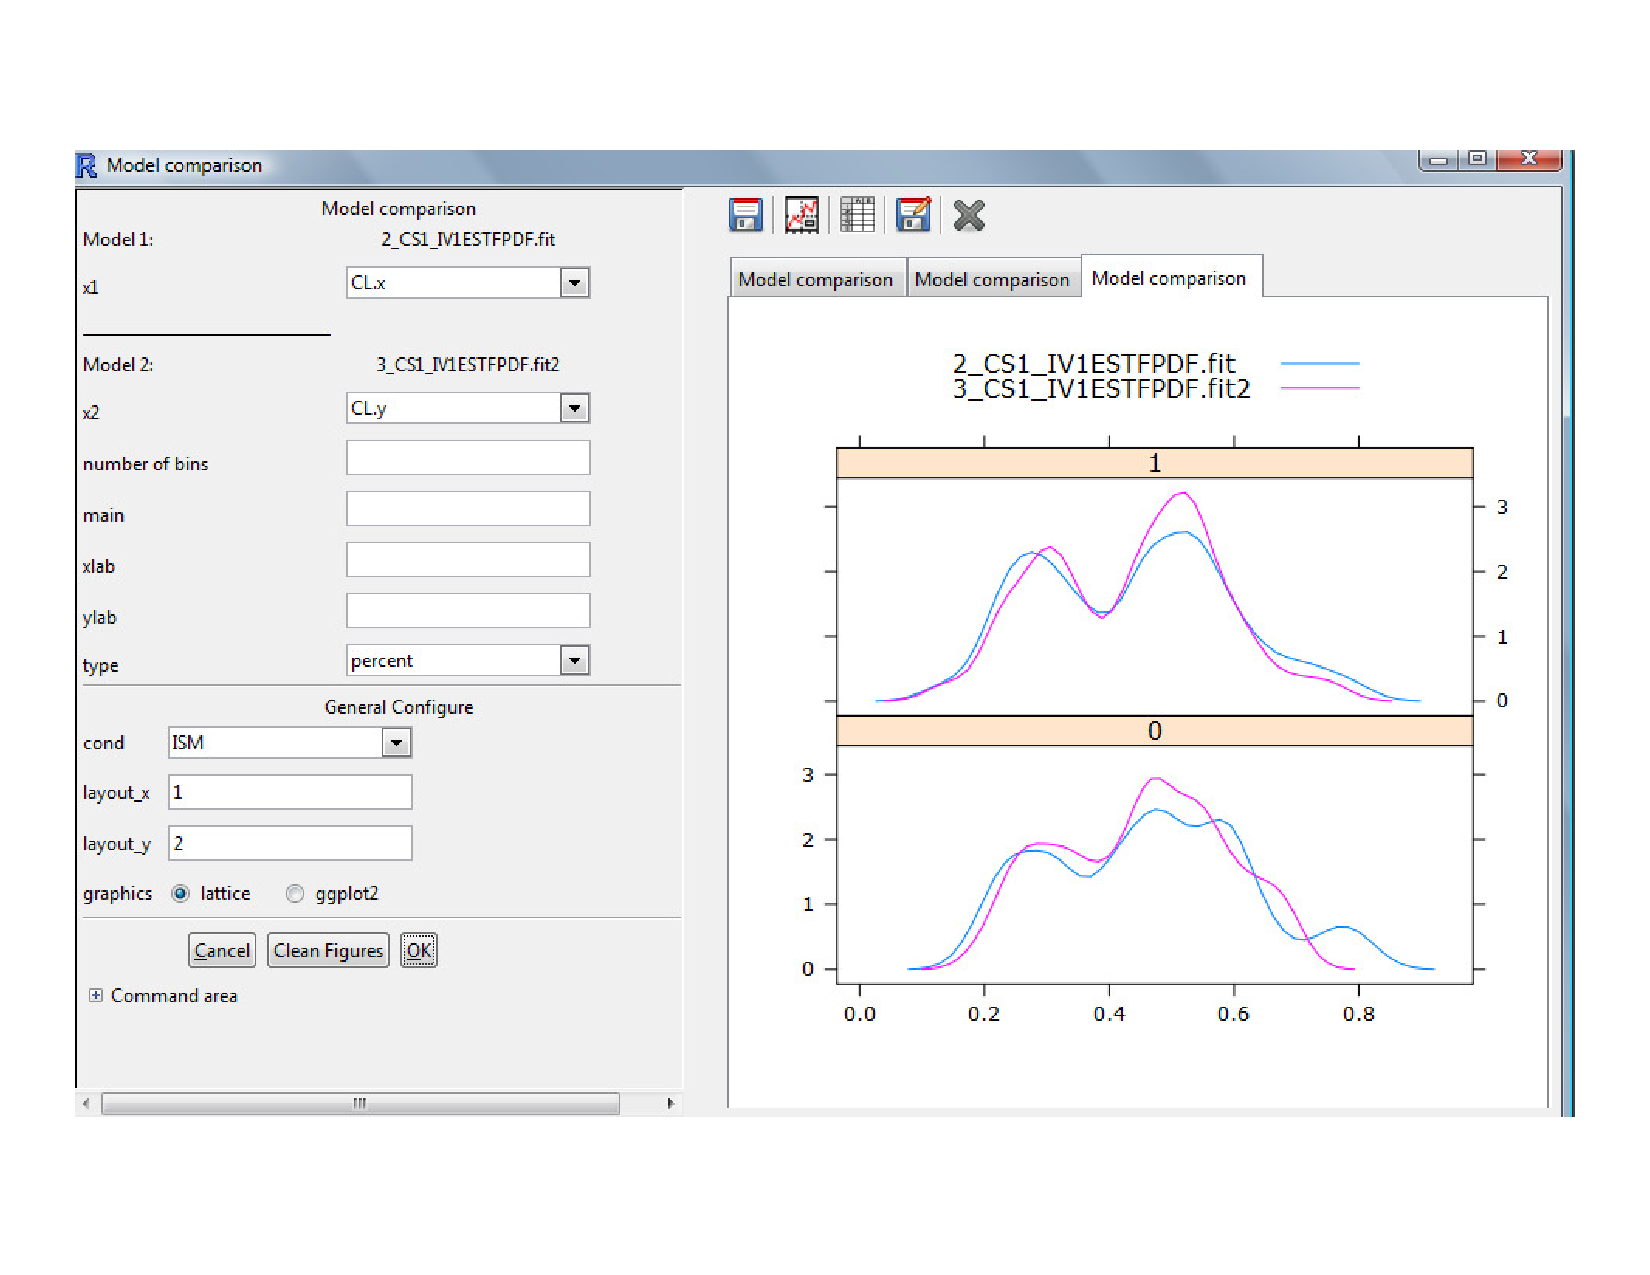
\includegraphics[scale=0.6]{modelcc2.pdf}
\caption{\textit{histogram comparison} for \textit{Model comparison}}
\label{modelcc2}
\end{figure}
%%%%%%%%%%%%%%%%%%%%%%%%%%%%%%%%%%%%%%%%%%%%%%%%%%%%%%%%%%%%%%%%%%%%%%%
\subsection{Interactive graphics}
This functional module incorporates a unique feature: interactive graphics into every step of model diagnostics. It targets to link diverse data sets in one integrative platform. Users can have access to this feature through \textit{ggobi} button in the graph interface. In addition, users have flexibility to apply this feature to achieve their specific goals. In the toolbar, there is option: \textit{interactive graphics}, designed for this purpose. It includes three steps: select datasets; configure mapping; and diagnostics. By linking diverse data sets with a key variable, users can seek patterns by brushing, linking and diagnosing patterns conveniently.
\newline
\newline
In ggobi, the main operation for brushing data is \textit{ctrl + b}. By moving the brushing rectangle, the users can select interesting subsets in ggobi. More information is available at \texttt{http:\\www.ggobi.org} if needed.
\section{Example}
One dataset from NONMEM is utilized to demonstrate PKgraph. This data set has 100 patients with covariates: ISM (gender), AGE, and WT. The data is fitted with one compartment model with zero order absorption and first order elimination.
\newline
\newline
As a text file, the fitting result from NONMEM is imported into PKgraph for further investigation and analysis. In the ``open'' dialog, we set up file format for reading with default parameters, and as a result, the input data shows up on the right panel while a message, ``Data is loaded successfully'' appears in the status bar at bottom of panel.
\newline
\newline
Alternatively, to make the input process flexible, users can input data into R first and then load data from ``Data from R environment'' in the ``open'' dialog. All the fitted results from a wide variety of software including NONMEM, SAS, etc can be loaded into this package.
\begin{verbatim}
> library(PKgraph)
> data(pkdata)
> PKgraph()
\end{verbatim}
\begin{figure}[h!tb]
\centering
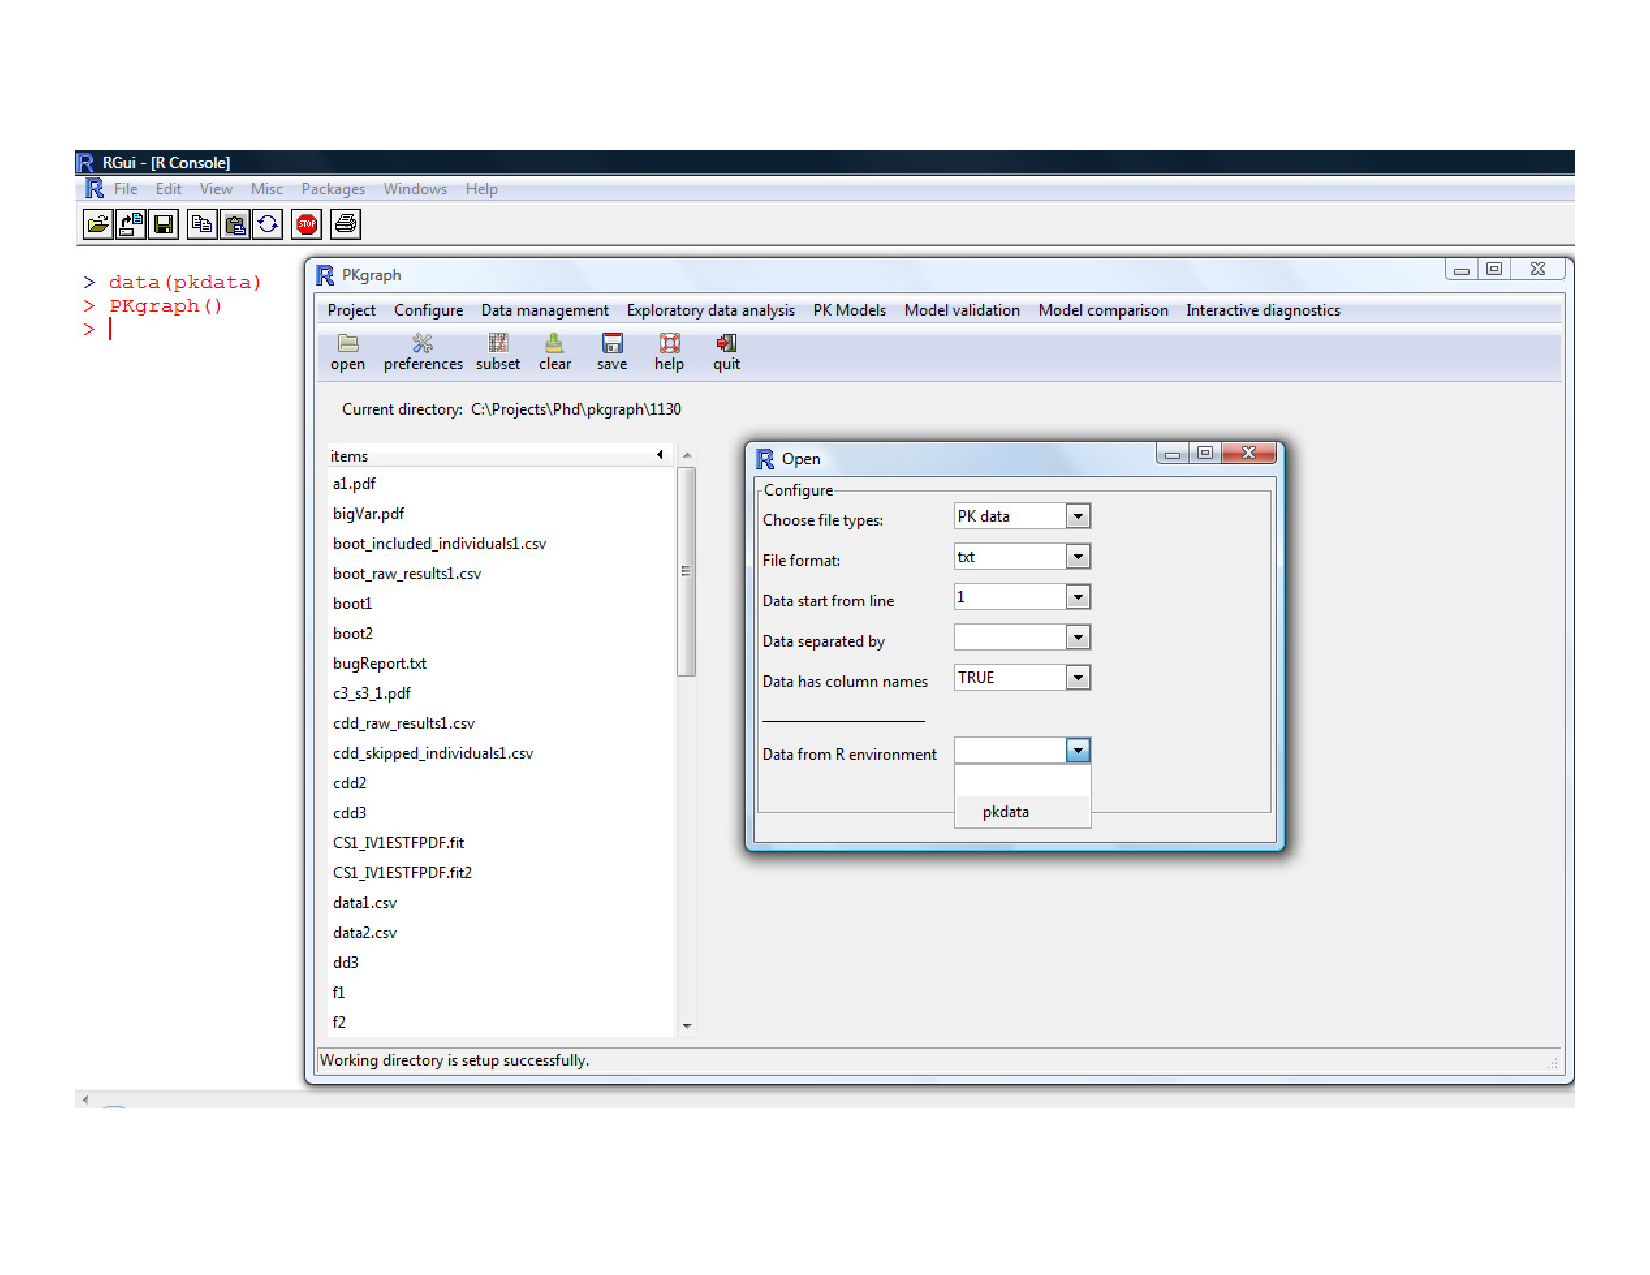
\includegraphics[scale=0.6]{inputData.pdf}
\caption{Load default data from ``Open'' dialog. After loading data with ``data(pkdata)'', users can select ``pkdata'' from Data from R environment in the ``Open'' dialog.}
\label{inputData}
\end{figure}
Figure~\ref{inputData} demonstrates how to load default data in the software.
\newline
\newline
To further explore data, first, we choose ``Bivariates'' from ``Exploratory Data Analysis'' located at menu bar to check the scatter plots of interested variables(Figure~\ref{c4_s2_5eda1}, Figure~\ref{c4_s2_5eda2}). The option ``cond'' from the functional model interface helps user to draw conditional plots to seek patterns for subgroups. Certainly, users can also select ``ggplot2'' graphic package with different taste of figure. Next, we can take advantage of interactive techniques to look at maximum concentration by clicking second image button on the right panel. This will start ggobi and load related data. GGobi includes two windows: console window and plot window. In order to link figures together, users need to open all interested figures by ``Display'' option in the menu bar. The following figure clearly shows that maximum concentration comes from male patients (value: 1). To look at these data in detail, we go back to the figure graphical user interface and click third image button to check selected data set in ggobi. The selected data set pops up and links to patient with ID: 55. We repeat the same procedure for other variables to check patterns.
\begin{figure}[h!tb]
\centering
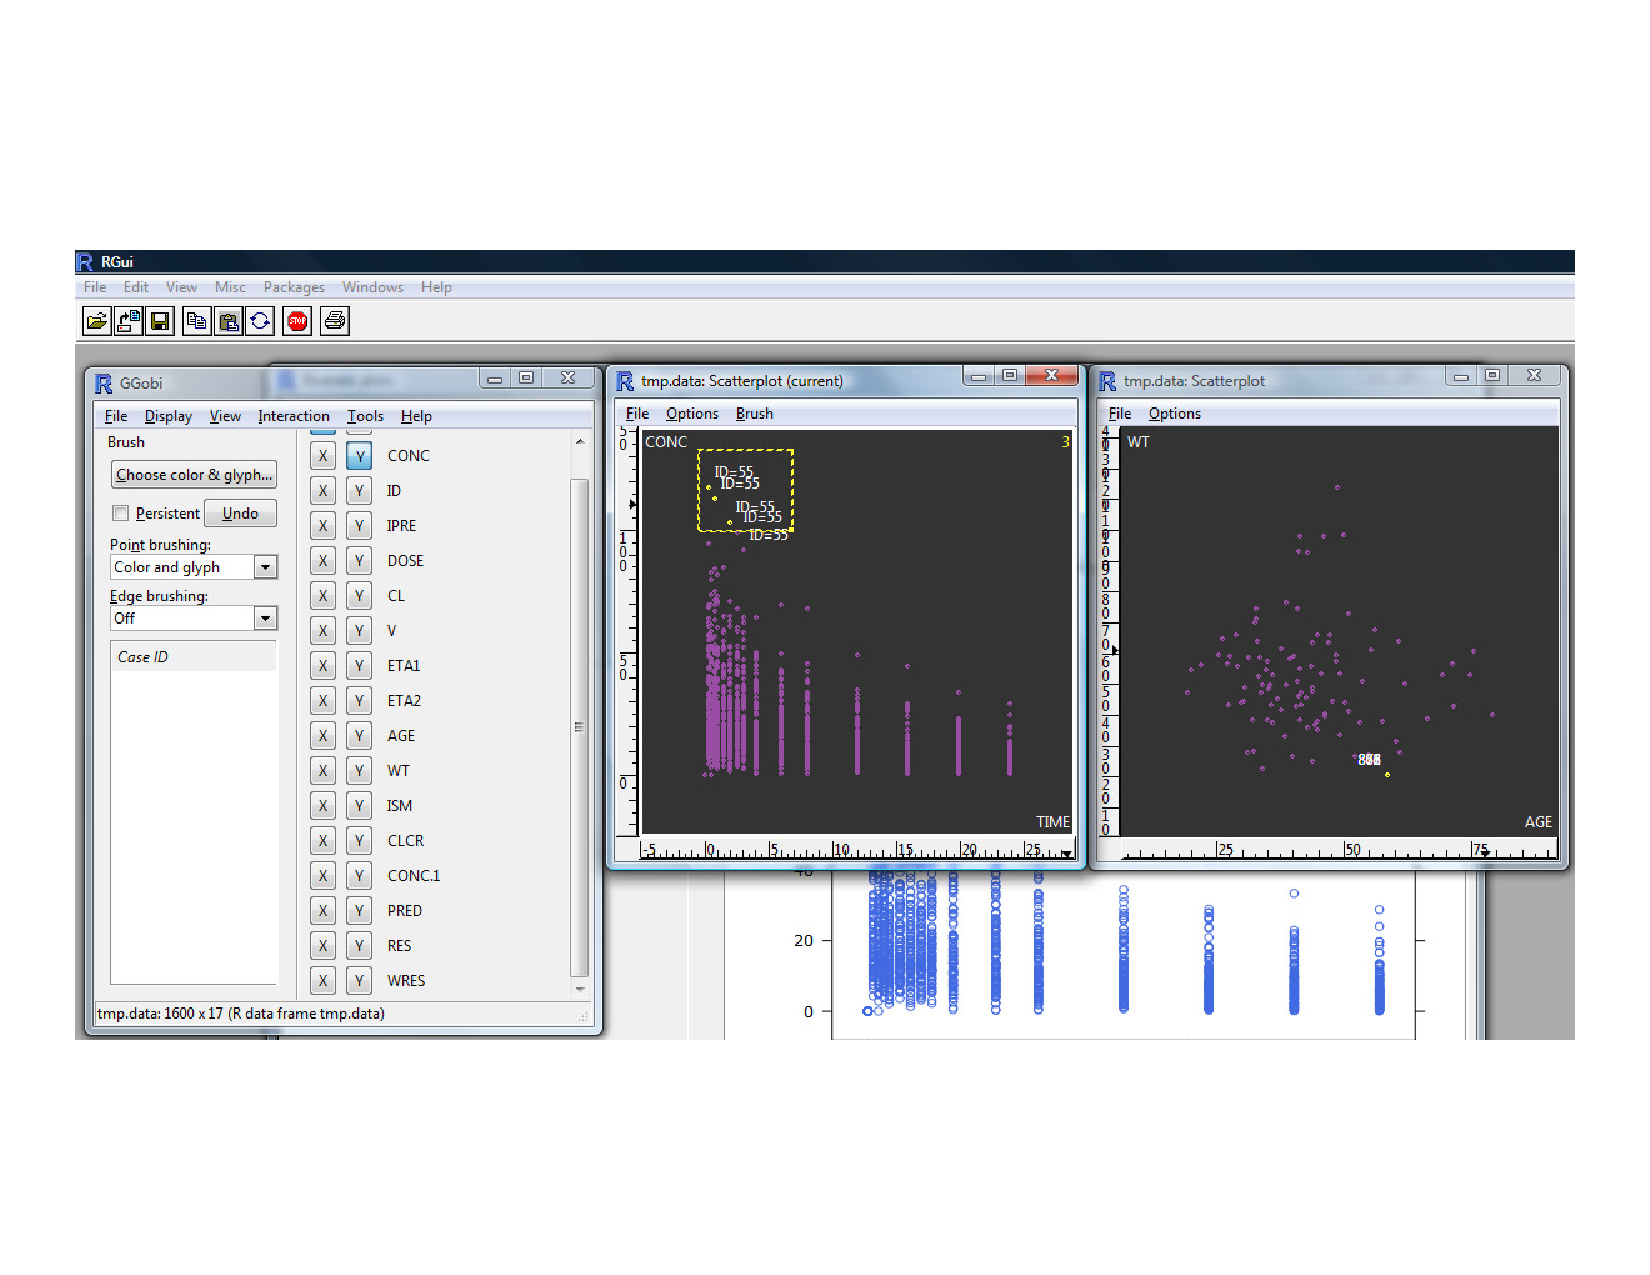
\includegraphics[scale=0.6]{c4_s2_5eda1.pdf}
\caption{Exploratory data analysis. Peak is identified with brushing. This patient is from light weight and middle age group.}
\label{c4_s2_5eda1}
\end{figure}
\begin{figure}[h!tb]
\centering
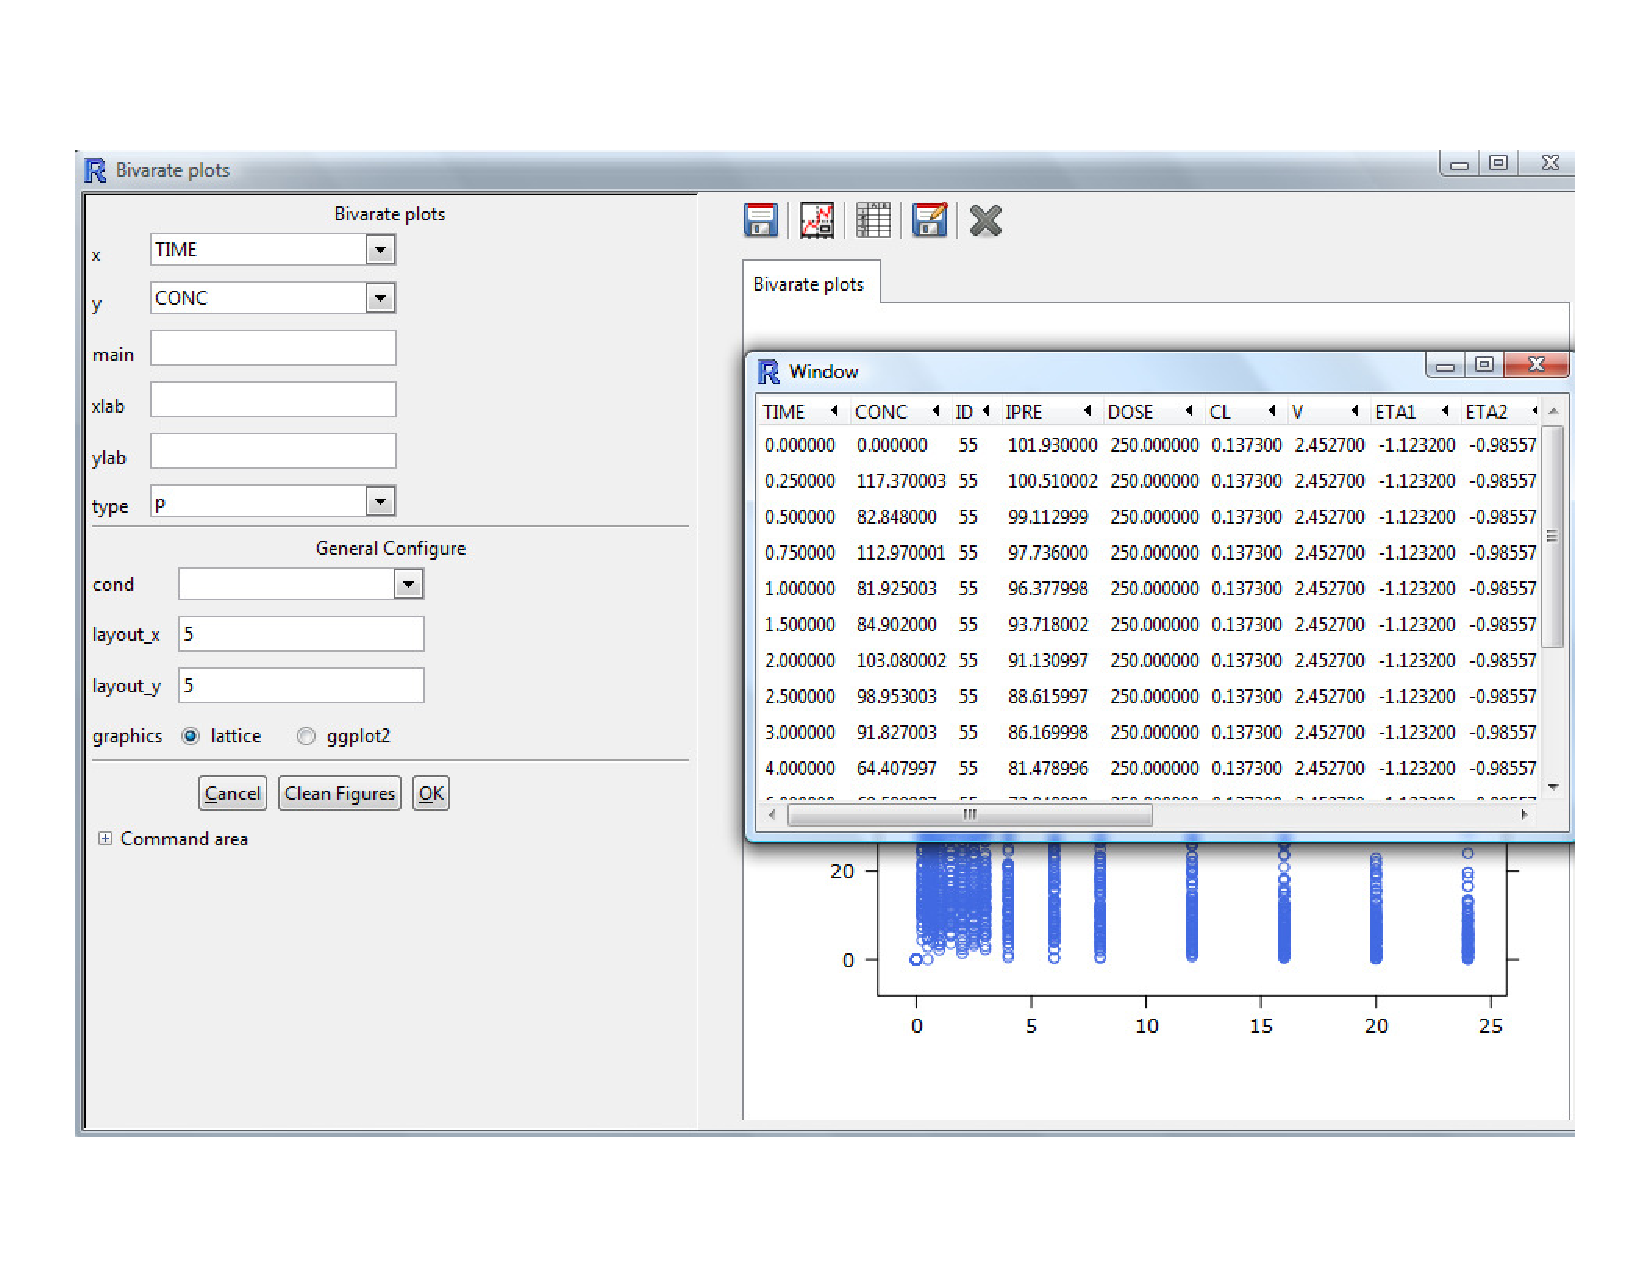
\includegraphics[scale=0.6]{c4_s2_5eda2.pdf}
\caption{Exploratory data analysis. The detailed information for this patient is selected for investigation.}
\label{c4_s2_5eda2}
\end{figure}
\newline
\newline
Next, we utilize ``PK model'' option to check model assumptions and diagnose model fitting. The program provides default names such as ID, TIME, COV, etc in order to automatically generate diagnosing results. After we match data variables to the default names, we can proceed to automatically generate routine goodness of fit plots for interested models. Figure ~\ref{c4_s2_6} is one of the results for structural model diagnostics.
\begin{figure}[h!tb]
\centering
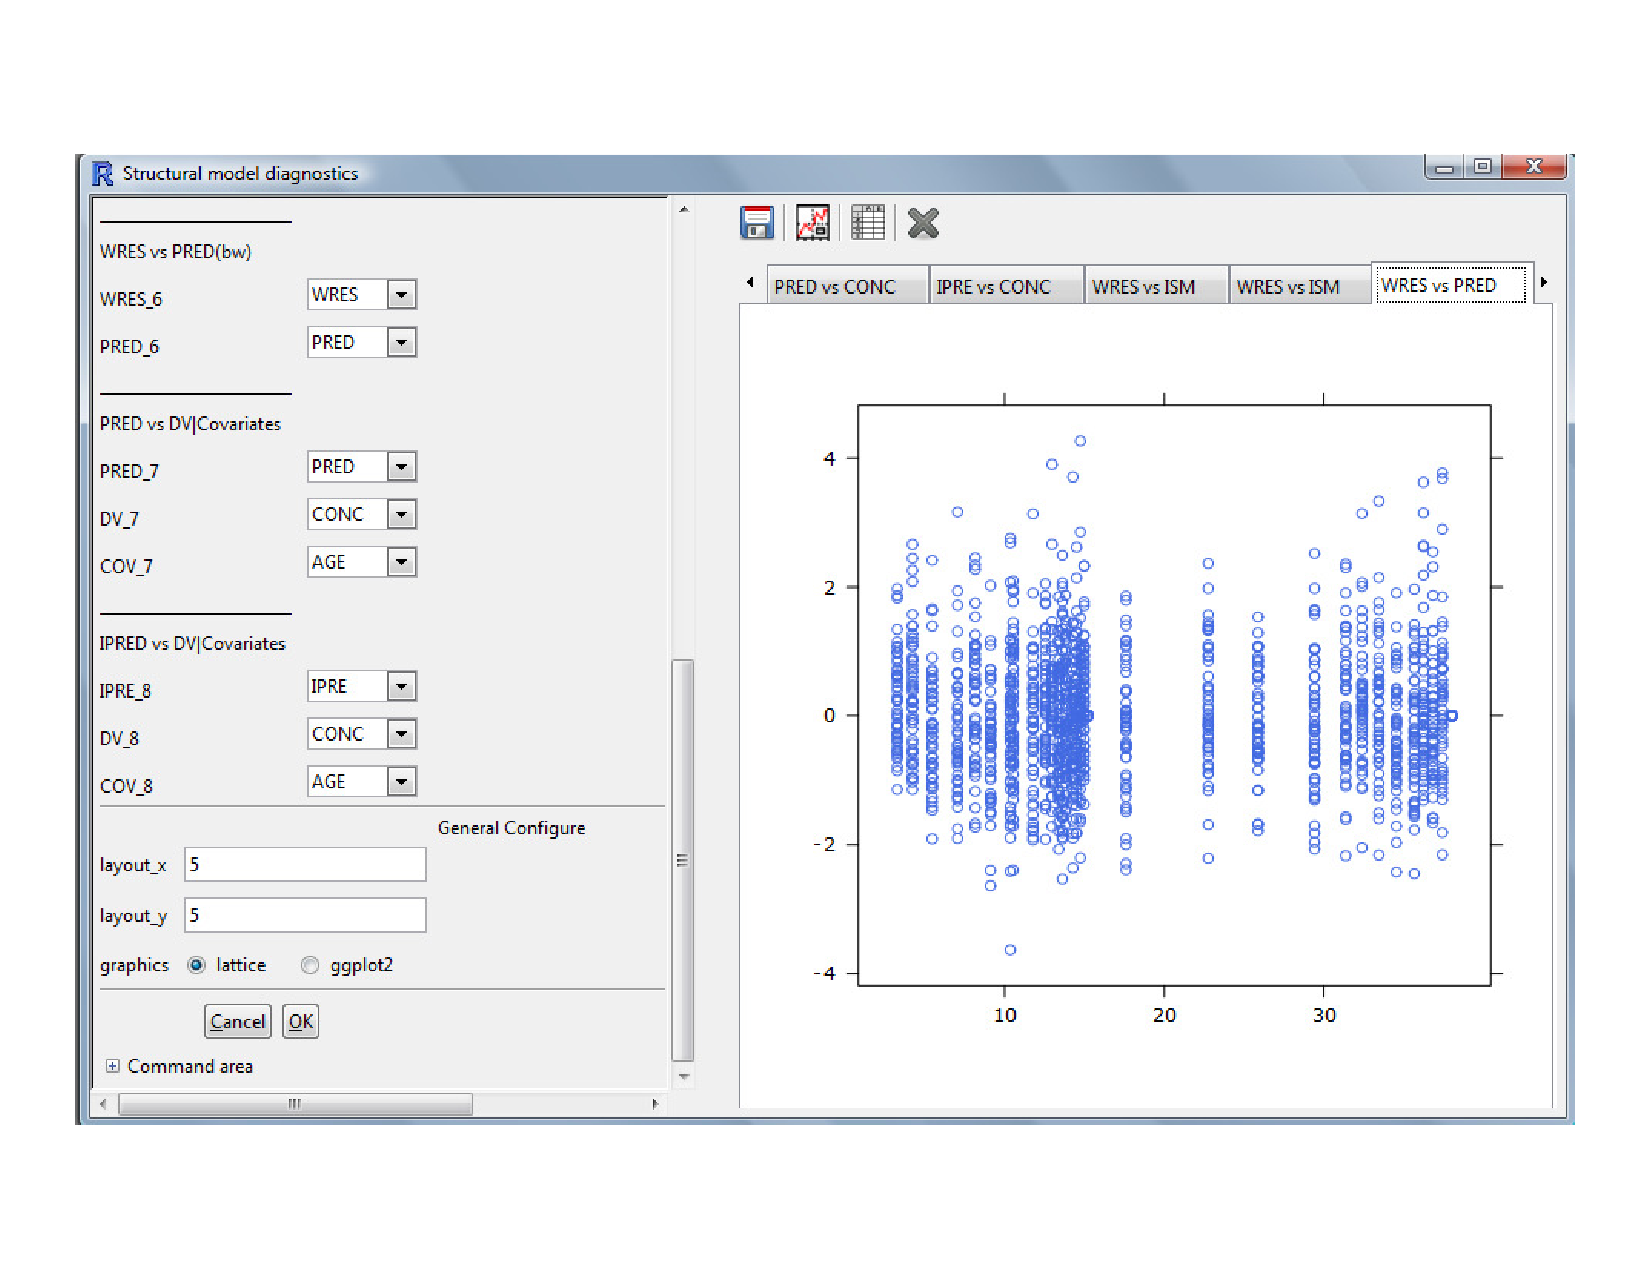
\includegraphics[scale=0.6]{c4_s2_6.pdf}
\caption{Structural model diagnostics.}
\label{c4_s2_6}
\end{figure}
\newline
\newline
To further look at the influential cases from same data set, we can link them together by ``model validation'' option in menu bar. In this process, we have 100 NONMEM runs available at directory: C:$\backslash$ Projects$\backslash$modelfit\_dir1 using PsN function: cdd. Let's input the path of these NONM runs, and select plot variable as ``CL''. After clicking ``OK'', we will have the parallel coordinates plot showing the CL variables for all NONMEM runs. From Figure ~\ref{c4_s2_7}, we can see some patients have more influential effects on CL when records from these patients are deleted.
\begin{figure}[h!tb]
\centering
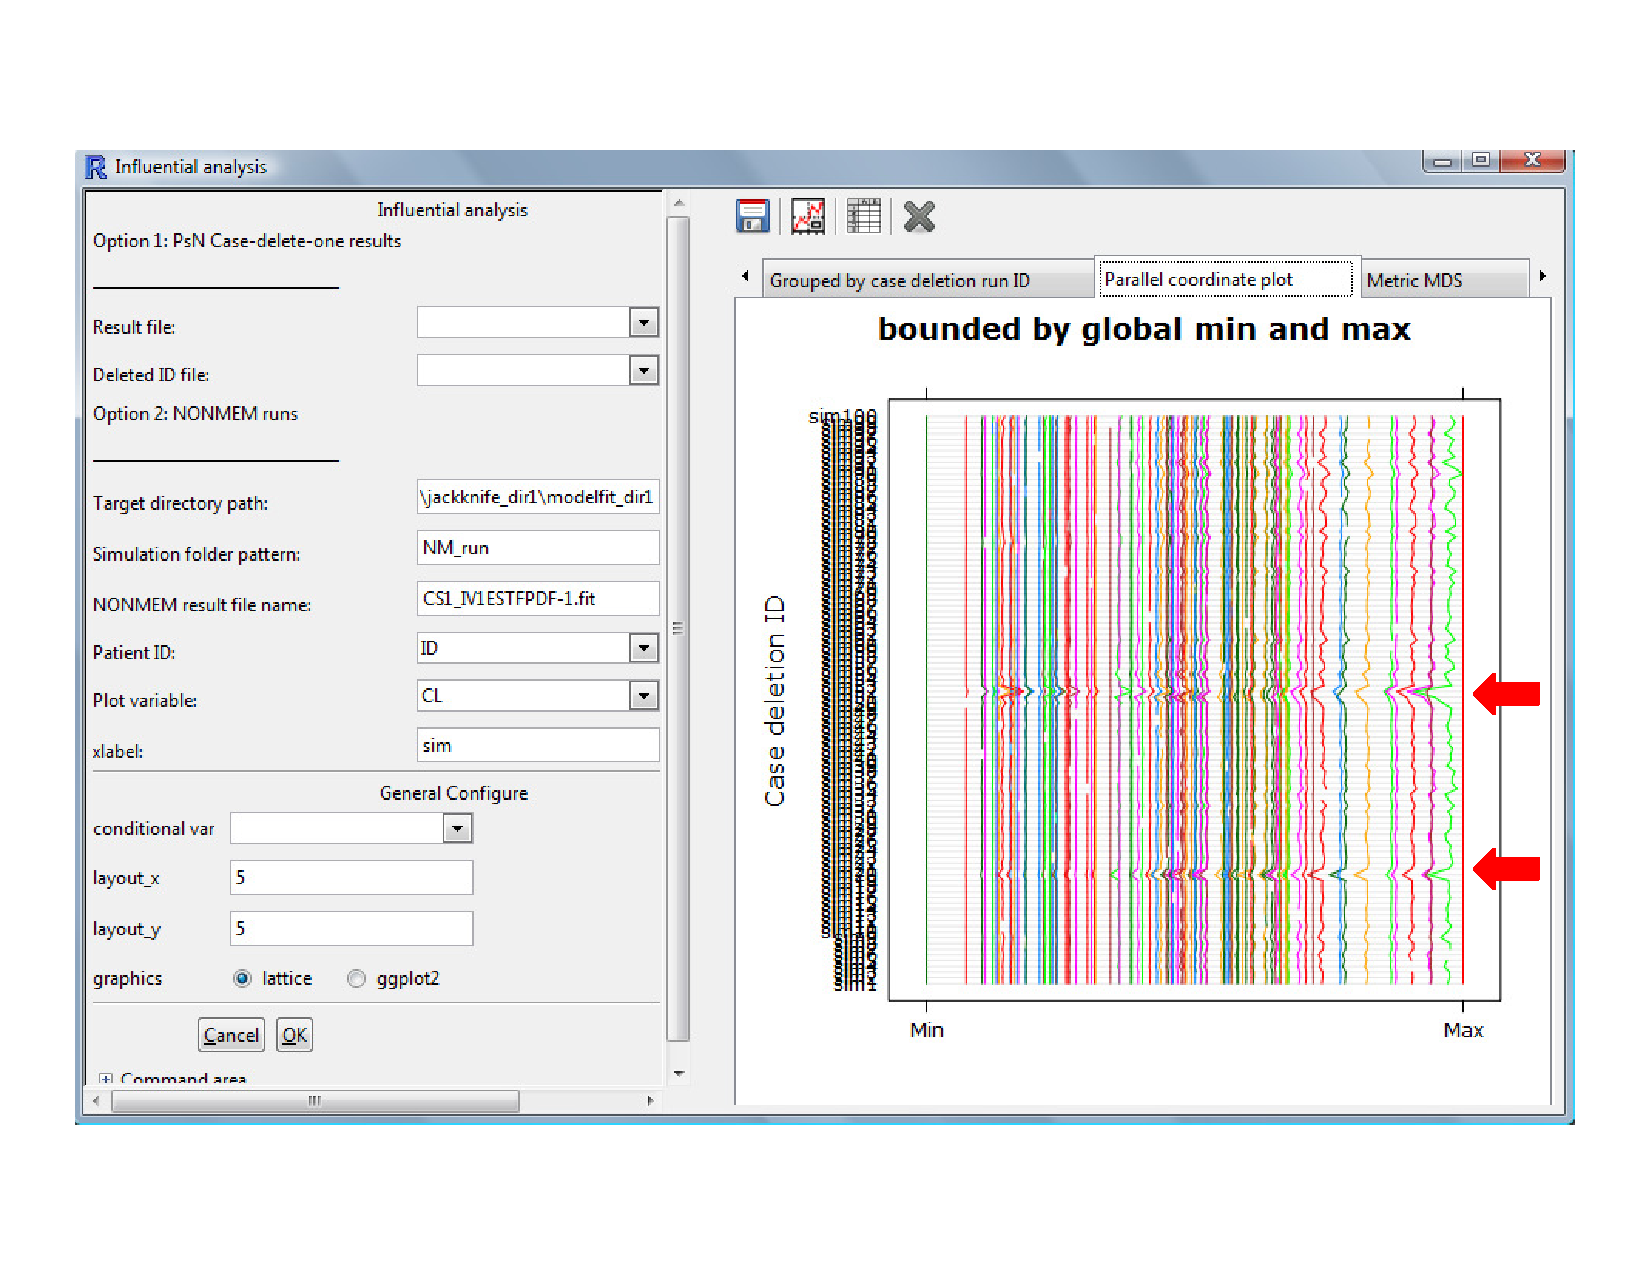
\includegraphics[scale=0.6]{c4_s2_7.pdf}
\caption{Influence analysis}
\label{c4_s2_7}
\end{figure}
\newline
\newline
Let's identify these influential cases with interactive graphics. Figure ~\ref{c4_s2_8} clearly demonstrates that these influential cases come from patient 52 and 20 based on multidimensional scaling and parallel coordinate plots.
\begin{figure}[h!tb]
\centering
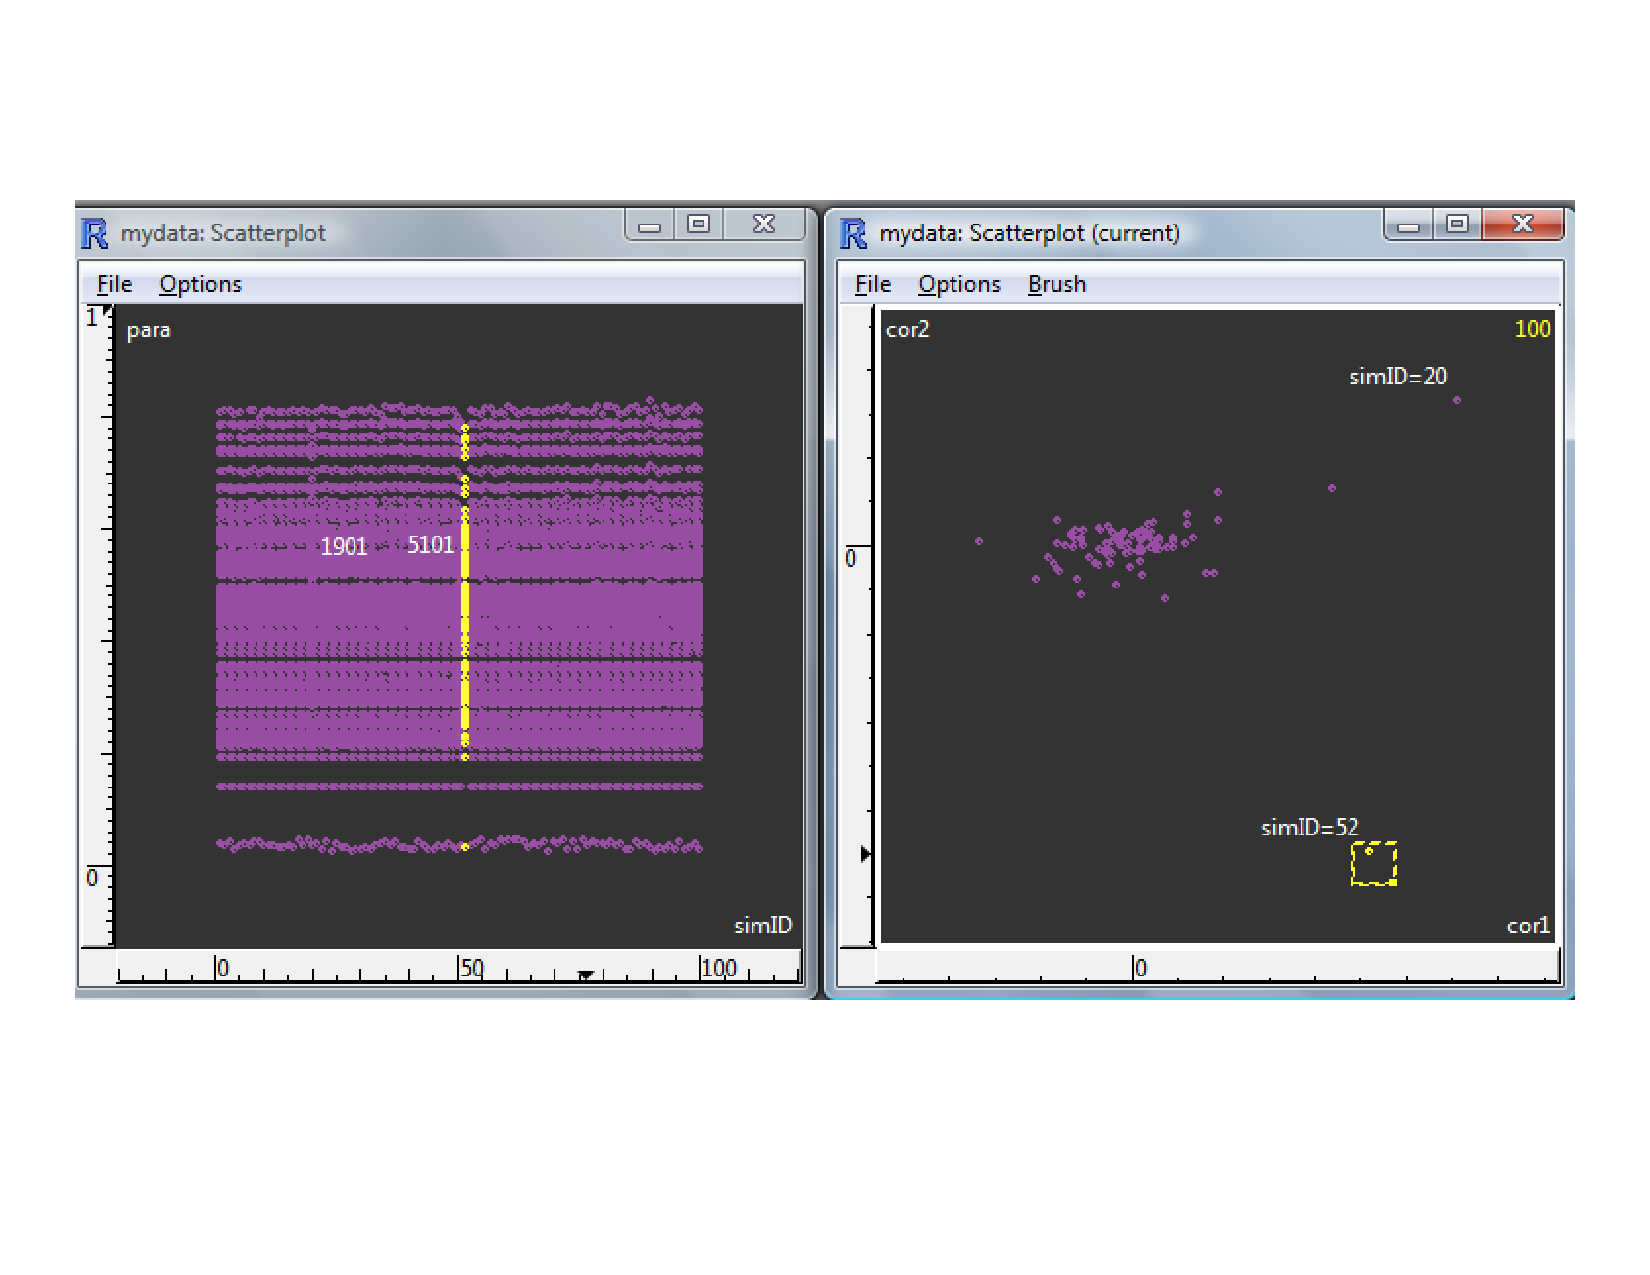
\includegraphics[scale=0.6]{c4_s2_8.pdf}
\caption{Influence analysis: linking results from multidimensional scaling and parallel coordinate plots.}
\label{c4_s2_8}
\end{figure}
\newline
\newline
In addition, we compare additive error model (2\_CS1\_IV1ESTFPDF.fit) with proportional error model (3\_ CS1\_IV1ESTFPDF.fit2) by ``model comparison'' function in the menu bar. By comparing the distribution of two models, Figure ~\ref{c4_s2_9} does not find significant difference between two models for CL. In addition, using gender as a conditional variable, we found first model always gave a higher peak value for both male and female.
\begin{figure}[h!tb]
\centering
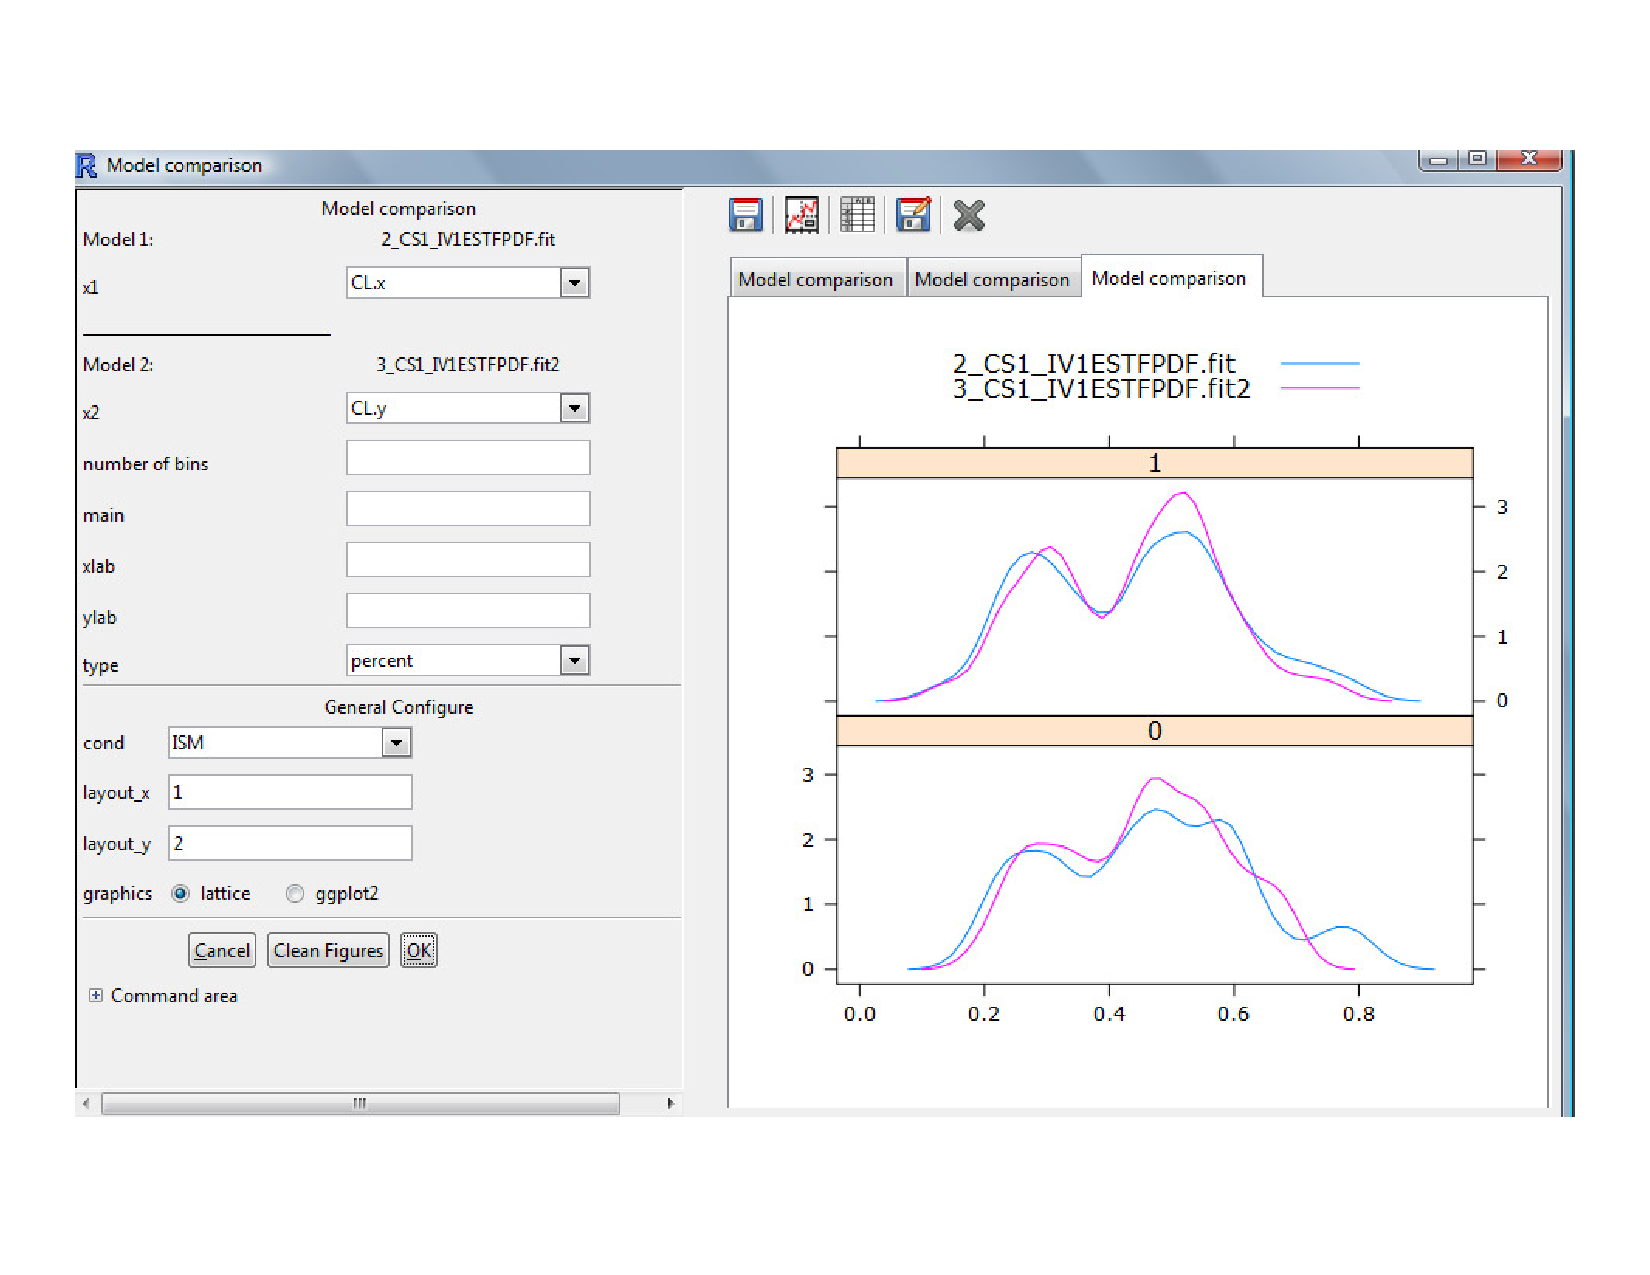
\includegraphics[scale=0.6]{modelcc2.pdf}
\caption{Histogram comparison for
comparing distributions of CL from two models.}
\label{c4_s2_9}
\end{figure}



\end{document}
